% Topic #4 - Cell Structure

%------------------------------------
% Main Settings
%------------------------------------
\documentclass[10pt]{beamer}

%--------------------------------------%
% Set font, and frame title info    %
%--------------------------------------%
\usefonttheme{serif}
\setbeamerfont{frametitle}{series=\bfseries}
\setbeamerfont{framesubtitle}{series=\bfseries}

%--------------------------------------
% "Sub-settings"
%--------------------------------------
\setbeamertemplate{navigation symbols}{}		% Get rid of navigation symbols
\setbeamertemplate{items}[default]				% Uses triangles and numbers instead of 3D balls (which I don't like)
\setbeamertemplate{itemize items}[circle]		% Use circles instead of triangles for itemized lists
\setbeamertemplate{footline}[frame number]      % Show frame #

%-------------------------------------
% Custom Commands
%-------------------------------------
\newtheorem{hypothesis}{Hypothesis}

%---For Footnotes---%
\usepackage{tikz}
\usepackage[absolute,overlay]{textpos}
\usetikzlibrary{calc,shapes.callouts,shapes.arrows,shapes,positioning}
\newenvironment{reference}[2]{%
	\begin{textblock*}{\textwidth}(#1,#2)
		\tiny\bgroup\color{gray}}{\egroup\end{textblock*}}
%------%		

%----------------------------------------%
% For making definitions in boxes        %
%----------------------------------------%
\usepackage{tcolorbox}

%--- For links ---%
\usepackage{hyperref}

%-- Packages for making nice tables --%
\usepackage{booktabs}
\usepackage{makecell}  % Required for specifying multiple rows within a table cell

%--------------------------------%
%     Custom Colours             %
%--------------------------------%
\usepackage{xcolor}
\definecolor{myblue}{rgb}{0,0.3,0.6}
\definecolor{myblue2}{rgb}{0,0.4,0.8}
\setbeamercolor{frametitle}{fg=myblue}
\setbeamercolor{framesubtitle}{fg=myblue2}
\setbeamercolor{itemize item}{fg=myblue}
\setbeamercolor{itemize subitem}{fg=myblue2}
\setbeamercolor{enumerate item}{fg=myblue}
\setbeamercolor{enumerate subitem}{fg=myblue2}


%----------------------------------%
% Creating nice blocks             %
%----------------------------------%
\setbeamercolor{block title}{bg=myblue, fg=white} %bg=background, fg=foreground
\setbeamercolor{block body}{bg=myblue!20, fg=black} %bg=background, fg=foreground
\setbeamerfont*{block title}{family=\sffamily, series=\bfseries, size=\large}
\setbeamertemplate{blocks}[rounded][shadow=true]


%------------------------%
% For making callouts    %
%------------------------%
\tikzset{
  notice/.style  = { draw, rectangle callout, callout relative pointer={#1} },
}

%------------------------------------------
%  Begin Presentations
%------------------------------------------
\begin{document}


%-----------------------%
%  Title Slide          %
%-----------------------%
\begin{frame}
	\begin{tikzpicture}[remember picture,overlay]
		\fill[color=myblue, draw=none] (current page.west) rectangle(current page.north east);
		\node at (2.0, 0.2) {\color{white}\LARGE{\textbf{Cell Structure}}};
	\end{tikzpicture}
\end{frame}


%-----------------------------%
%  Basic Unit of Life         %
%-----------------------------%
\begin{frame}[t]
\vspace{0.5cm}	

	\begin{center}
		\textcolor{myblue}{Cells are the basic unit of life!}\\
	\end{center}
	
	\vspace{0.5cm}

	Smallest unit of living things:
		\medskip
		\begin{itemize}
			\item Single-celled organisms are the smallest units of life
			\medskip
			\item Are the basic units of multi-cellular organisms
		\end{itemize}	
\end{frame}


%-----------------------------%
%  Basic Unit of Life II      %
%-----------------------------%
\begin{frame}[t]	

	\begin{reference}{4mm}{92mm}
		\rule{1.5cm}{0.25pt}\\
		Tree from Hug et al. (2016) \emph{Nature Microbiology} \textbf{1}: 16048.
	\end{reference}
	
	\begin{center}
		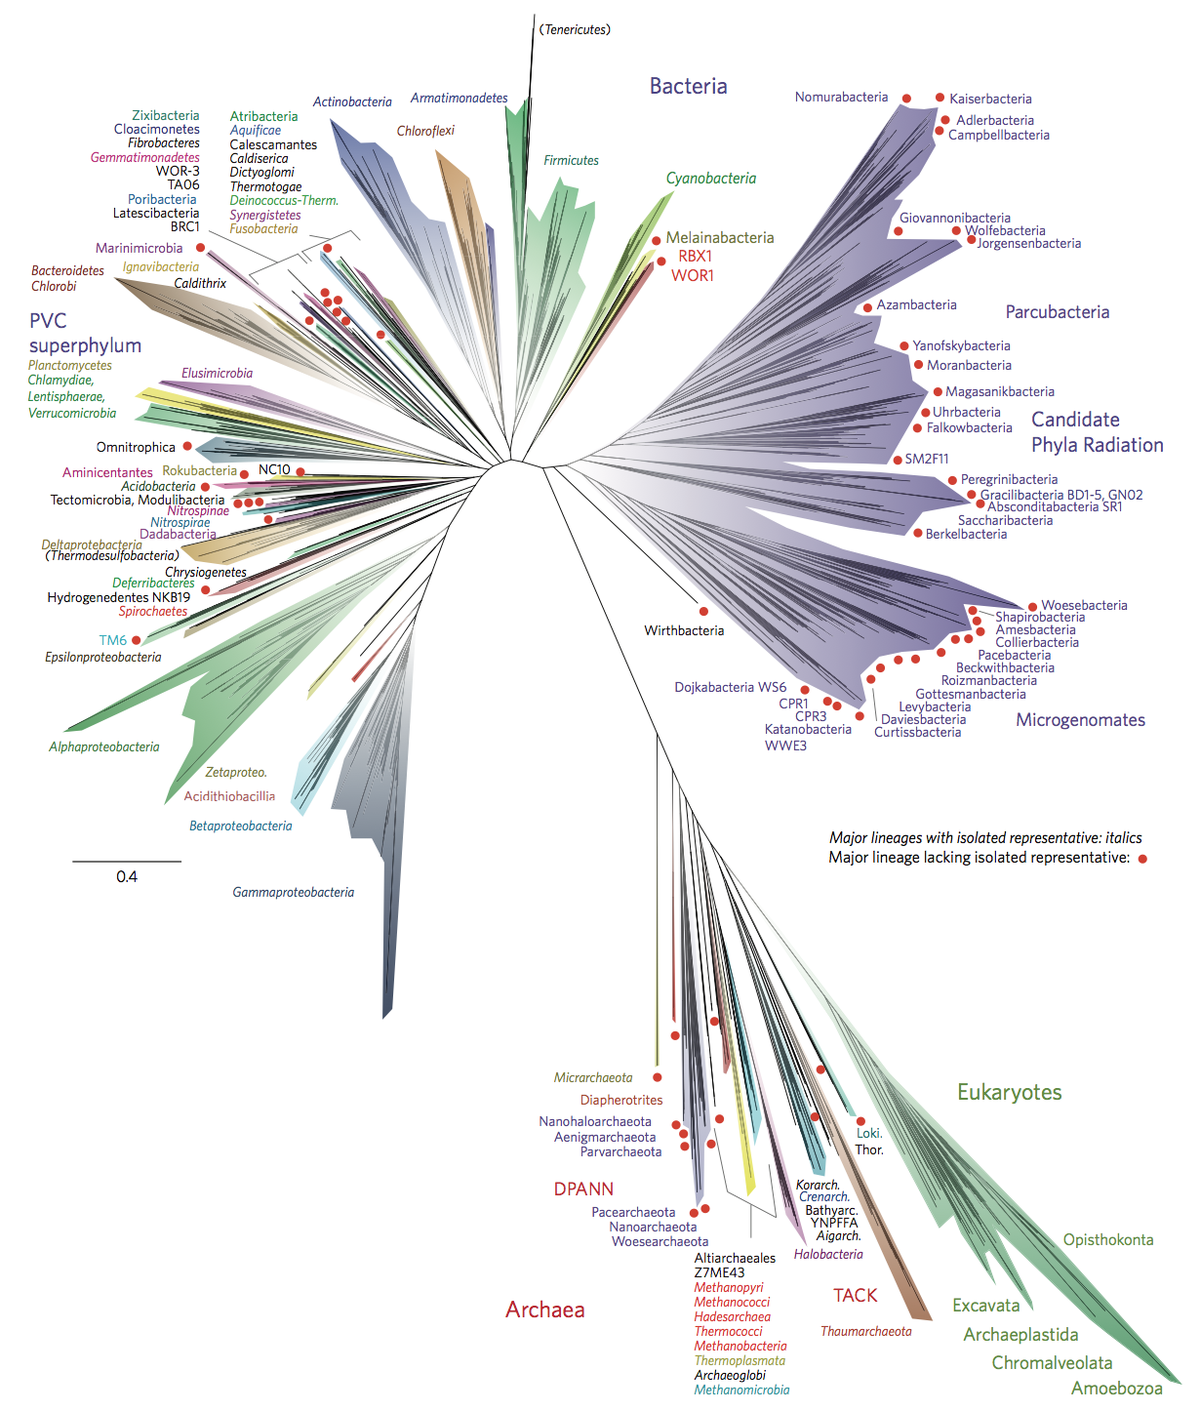
\includegraphics[width=0.6\textwidth]{figures/tree.png}
	\end{center}
\end{frame}


%-----------------------------%
%  Basic Unit of Life III     %
%-----------------------------%
\begin{frame}[t]	

	\begin{center}
		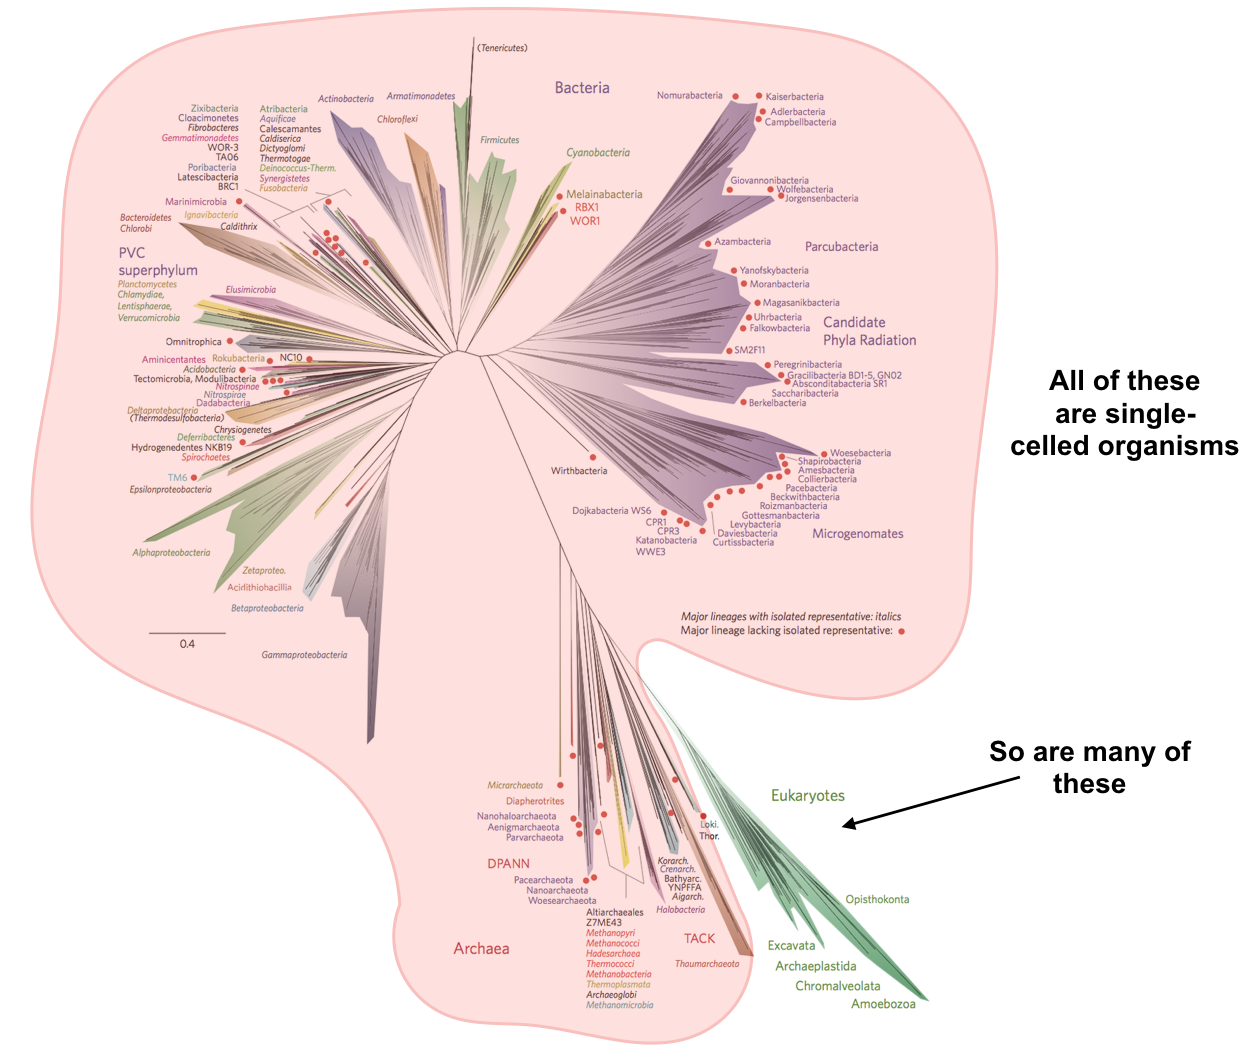
\includegraphics[width=0.8\textwidth]{figures/tree2.png}
	\end{center}
\end{frame}


%-----------------------------%
%  Basic Unit of Life IV      %
%-----------------------------%
\begin{frame}[t]	
\frametitle{Basic Unit of Life}

	\begin{columns}
		\begin{column}{0.8\textwidth}
			In single-celled organisms, importance of the cell is obvious.
		\end{column}
		
		\begin{column}{0.2\textwidth}
			\begin{center}
				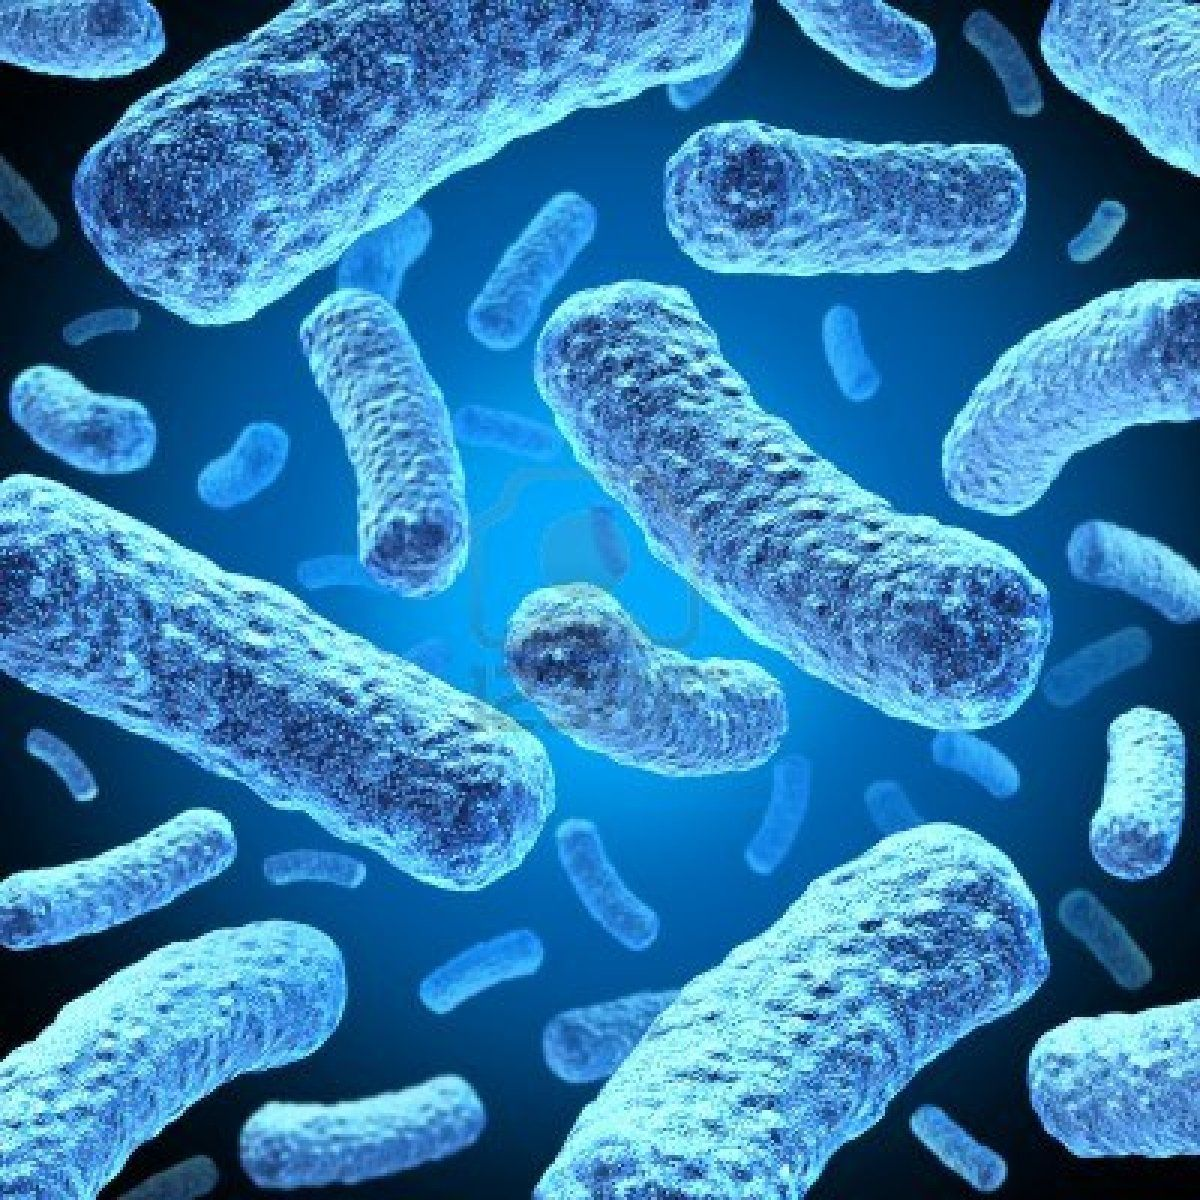
\includegraphics[width=0.9\textwidth]{figures/bacteria.jpg}\\
			\end{center}
		\end{column}
	\end{columns}
	
	\vspace{1.0cm}
	
	In multi-cellular organisms, they are the basic unit of organization.
	
		\begin{center}
			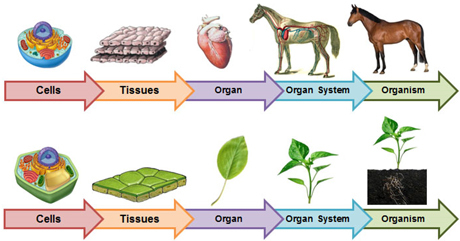
\includegraphics[width=0.6\textwidth]{figures/systems.jpg}
		\end{center}
\end{frame}


%-----------------------------%
%  Basic Unit of Life V       %
%-----------------------------%
\begin{frame}[t]	
\frametitle{Basic Unit of Life}

	\begin{tikzpicture}[overlay]
		%- Images -%
		\node at (1.0, -0.5) (cell) {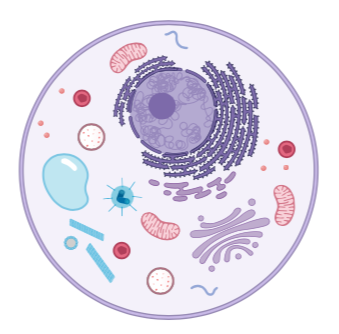
\includegraphics[width=0.1\textwidth]{figures/cell.png}};
		\node at (1.0, -2.0) (tissue) {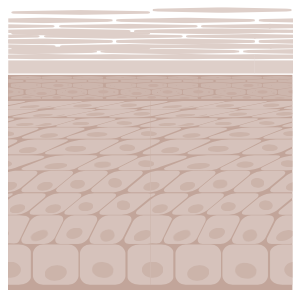
\includegraphics[width=0.08\textwidth]{figures/tissue.png}};
		\node at (1.0, -3.5) (organ) {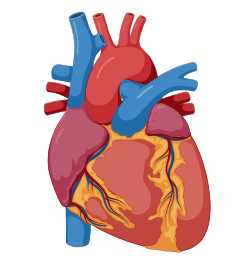
\includegraphics[width=0.1\textwidth]{figures/organ.png}};
		\node at (1.0, -5.0) (system) {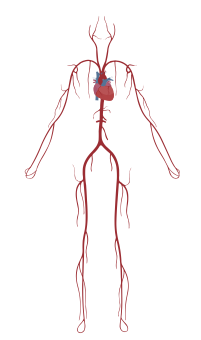
\includegraphics[width=0.1\textwidth]{figures/organsystem.png}};
		\node at (1.0, -6.5) (organism) {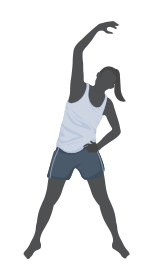
\includegraphics[width=0.1\textwidth]{figures/organism.png}};
		
		%- Types -%
		\node[draw=myblue2, fill=myblue2!30, rounded corners, text width=1.5cm, align=center] at (4.0, -0.5) (cell2) {Cell};
		\node[draw=myblue2, fill=myblue2!30, rounded corners, text width=1.5cm, align=center] at (4.0, -2.0) (tissue2) {Tissue};
		\node[draw=myblue2, fill=myblue2!30, rounded corners, text width=1.5cm, align=center] at (4.0, -3.5) (organ2) {Organ};
		\node[draw=myblue2, fill=myblue2!30, rounded corners, text width=1.5cm, align=center] at (4.0, -5.0) (system2) {Organ System};
		\node[draw=myblue2, fill=myblue2!30, rounded corners, text width=1.5cm, align=center] at (4.0, -6.5) (organism2) {Organism};
		
		\draw[->, >=latex, thick] (cell2) -- (tissue2);
		\draw[->, >=latex, thick] (tissue2) -- (organ2);
		\draw[->, >=latex, thick] (organ2) -- (system2);
		\draw[->, >=latex, thick] (system2) -- (organism2);
		
		%- Definitions -%
		\node[text width=5cm] at (8.0, -0.5) (cell3) {Smallest unit that can carry out life's activities};
		\node[text width=5cm] at (8.0, -2.0) (tissue3) {Group of \emph{\textcolor{myblue}{cells}} working together to perform a specific job};
		\node[text width=5cm] at (8.0, -3.5) (organ3) {Group of \emph{\textcolor{myblue}{tissues}} working together to perform a specific job};
		\node[text width=5cm] at (8.0, -5.0) (systen3) {Group of \emph{\textcolor{myblue}{organs}} working together to perform a specific job};
		\node[text width=5cm] at (8.0, -6.5) (organism3) {Group of \emph{\textcolor{myblue}{systems}} working together to perform a specific job};
	\end{tikzpicture}	
\end{frame}


%------------------------------%
% Cellular Membrane            %
%------------------------------%
\begin{frame}
	
	\begin{center}
		\LARGE{\textcolor{myblue}{The Cellular/Plasma Membrane}}
	\end{center}

\end{frame}


%------------------------------%
% Cellular Membrane I          %
%------------------------------%
\begin{frame}[t]
\frametitle{Cellular Membrane}
\vspace{0.5cm}

	\textbf{All} cells have a cellular membrane (also called a \emph{plasma} membrane)\\

	\vspace{0.5cm}
	
	Important for:
		\smallskip
		\begin{itemize}
			\item Controlling what goes in and out of the cell (\textcolor{myblue}{\emph{selective permeability}})
			\smallskip
			\item Maintaining internal conditions (\textcolor{myblue}{\emph{homeostasis}})
		\end{itemize}
	
	\begin{columns}
		\begin{column}{0.5\textwidth}
			\begin{center}
				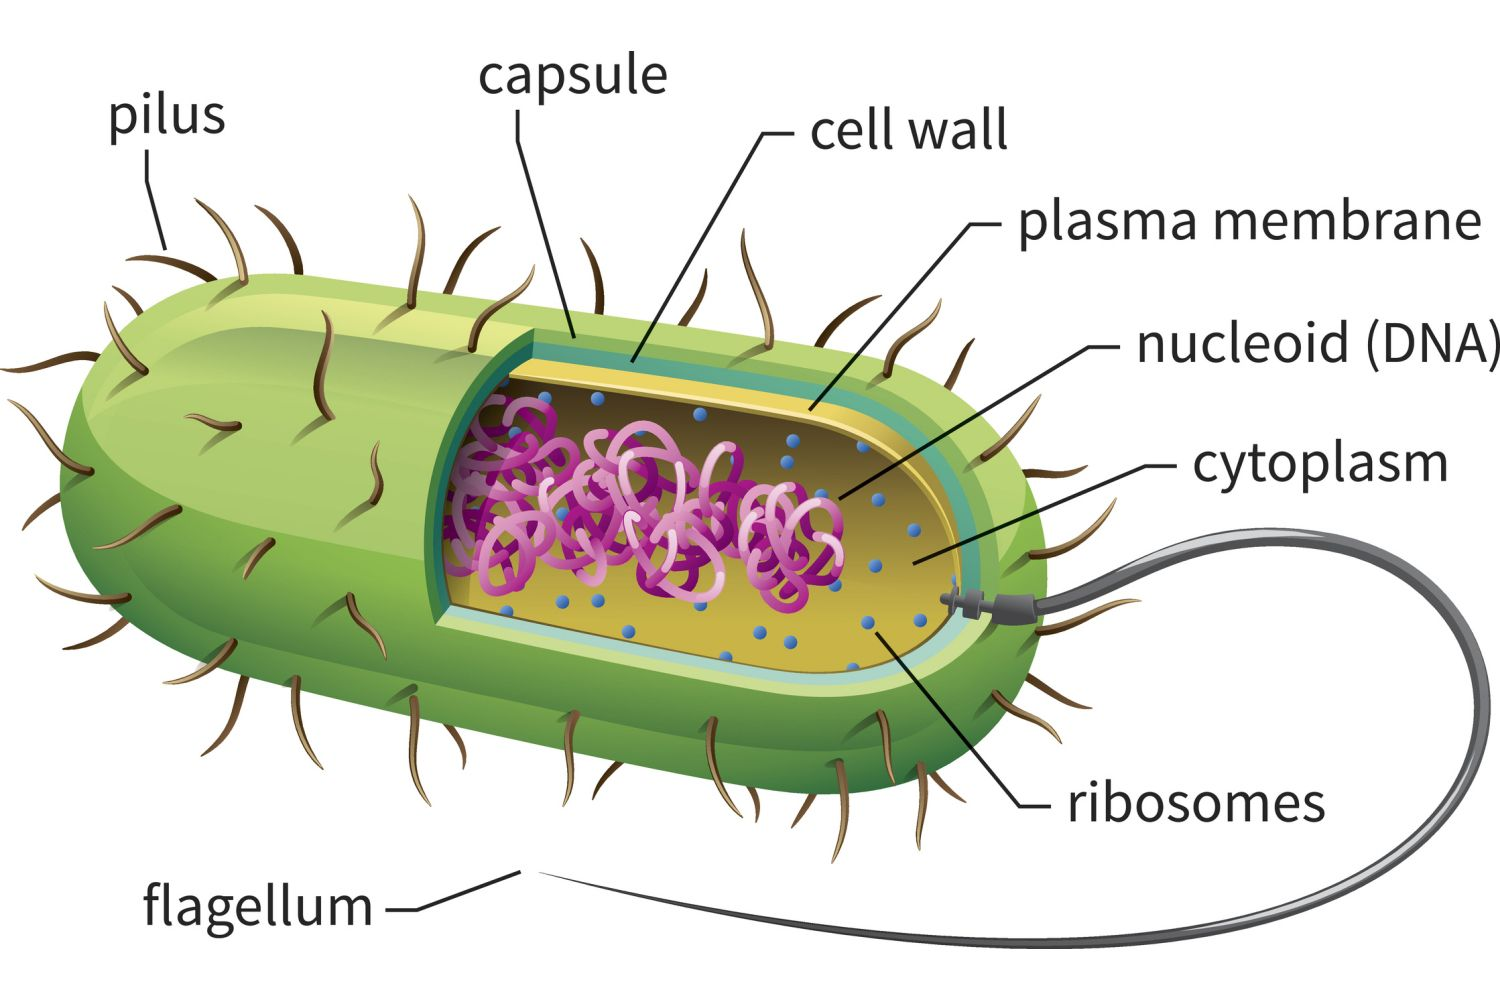
\includegraphics[width=0.8\textwidth]{figures/bacteria_cell.jpg}
			\end{center}	
		\end{column}
		
		\begin{column}{0.5\textwidth}
			\begin{center}
				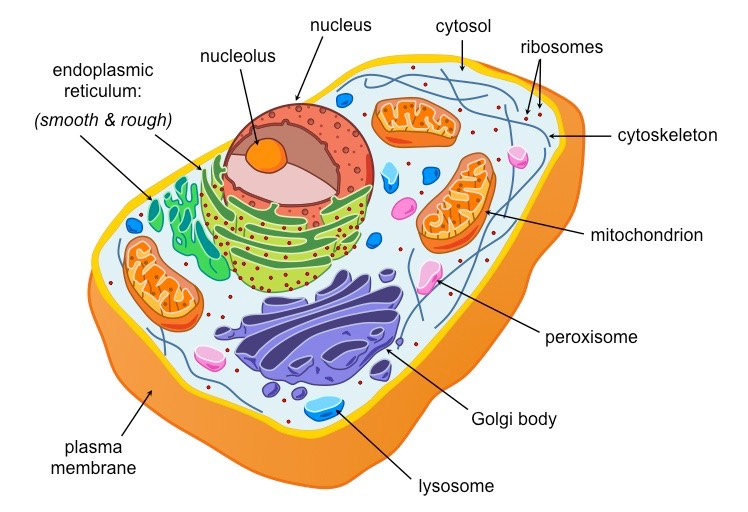
\includegraphics[width=0.8\textwidth]{figures/animal.jpg}
			\end{center}	
		\end{column}
	\end{columns}	
\end{frame}


%------------------------------%
% Cellular Membrane II         %
%------------------------------%
\begin{frame}[t]
\frametitle{Cellular Membrane}
\vspace{0.5cm}

	\begin{center}
		\begin{block}{Homeostasis}
			The steady-state equilibrium conditions (pH, ionic concentrations, temperature, etc.) required for a biological entity (cells, organs, organisms, etc.) to maintain its function.
		\end{block}
	\end{center}
\end{frame}


%------------------------------%
% Cellular Membrane III        %
%------------------------------%
\begin{frame}[t]
\frametitle{Cellular Membrane}
\vspace{0.5cm}

	``Like dissolves like''\\
	
	\medskip
	
		\begin{itemize}
			\item Polar things (\textbf{\textcolor{myblue}{hydrophilic}}) dissolve other polar things
			\medskip
			\item Non-polar things (\textbf{\textcolor{myblue}{hydrophobic}}) dissolve other non-polar things\\
		\end{itemize}
	
	\vspace{0.5cm}
	
	\begin{center}
		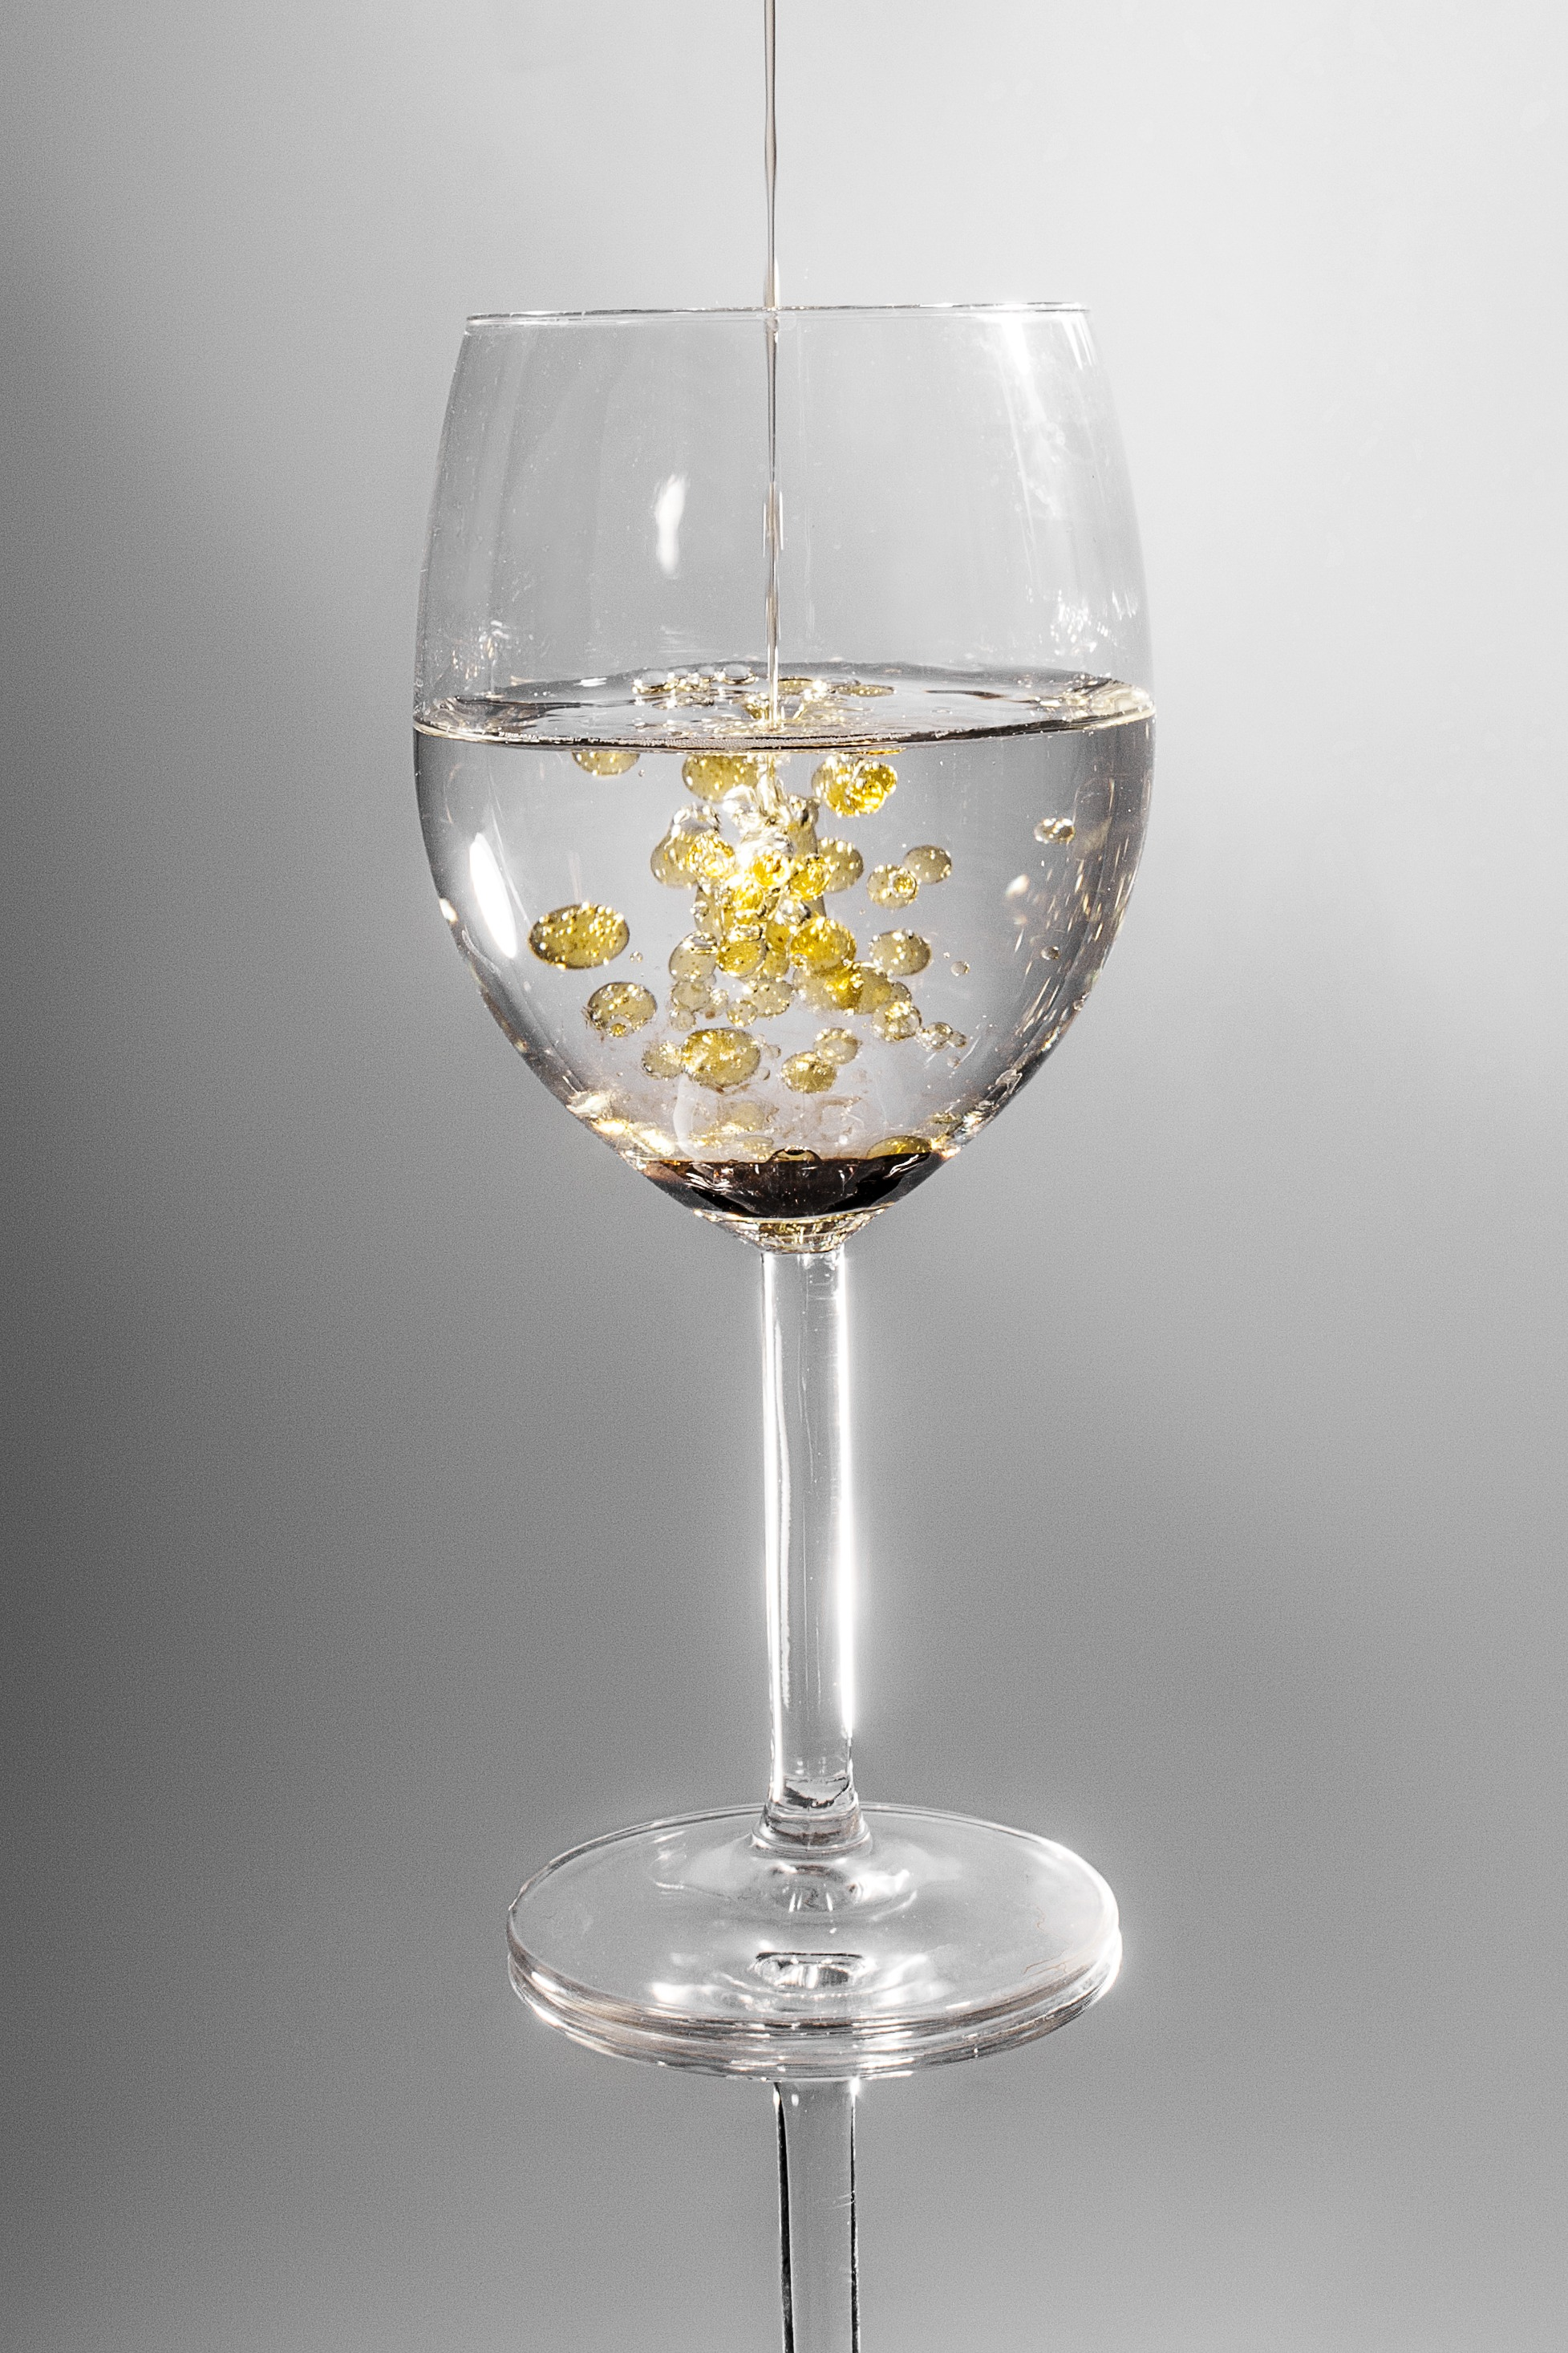
\includegraphics[width=0.3\textwidth]{figures/oil_water.jpg}
	\end{center}	
\end{frame}


%------------------------------%
% Cellular Membrane IV         %
%------------------------------%
\begin{frame}[t]
\frametitle{Cellular Membrane}
\vspace{0.5cm}

	So\ldots how do detergents work?
	
	\vspace{0.25cm}
	
	Goal:
		\begin{itemize}
			\item Make oils (hydrophobic) soluble in water (hydrophilic)
		\end{itemize}
	
	\vspace{0.5cm}
	
	\begin{columns}
		\begin{column}{0.5\textwidth}
			\centerline{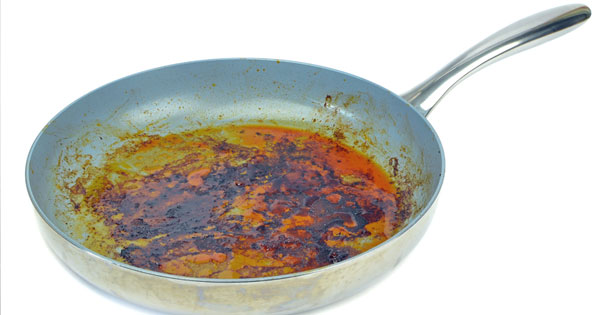
\includegraphics[width=0.7\textwidth]{figures/pan.jpg}}
		\end{column}
		
		\begin{column}{0.5\textwidth}
			\centerline{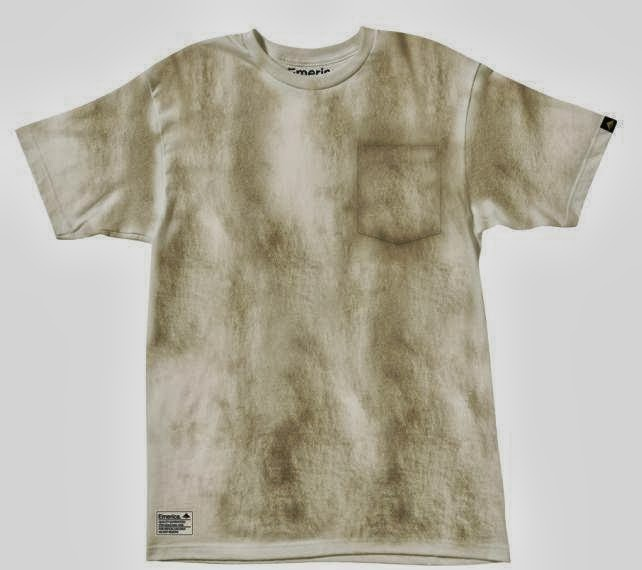
\includegraphics[width=0.7\textwidth]{figures/shirt.jpg}}
		\end{column}
	\end{columns}	
\end{frame}


%------------------------------%
% Cellular Membrane V          %
%------------------------------%
\begin{frame}[t]
\frametitle{Micelle}
\vspace{0.5cm}

	\begin{center}
		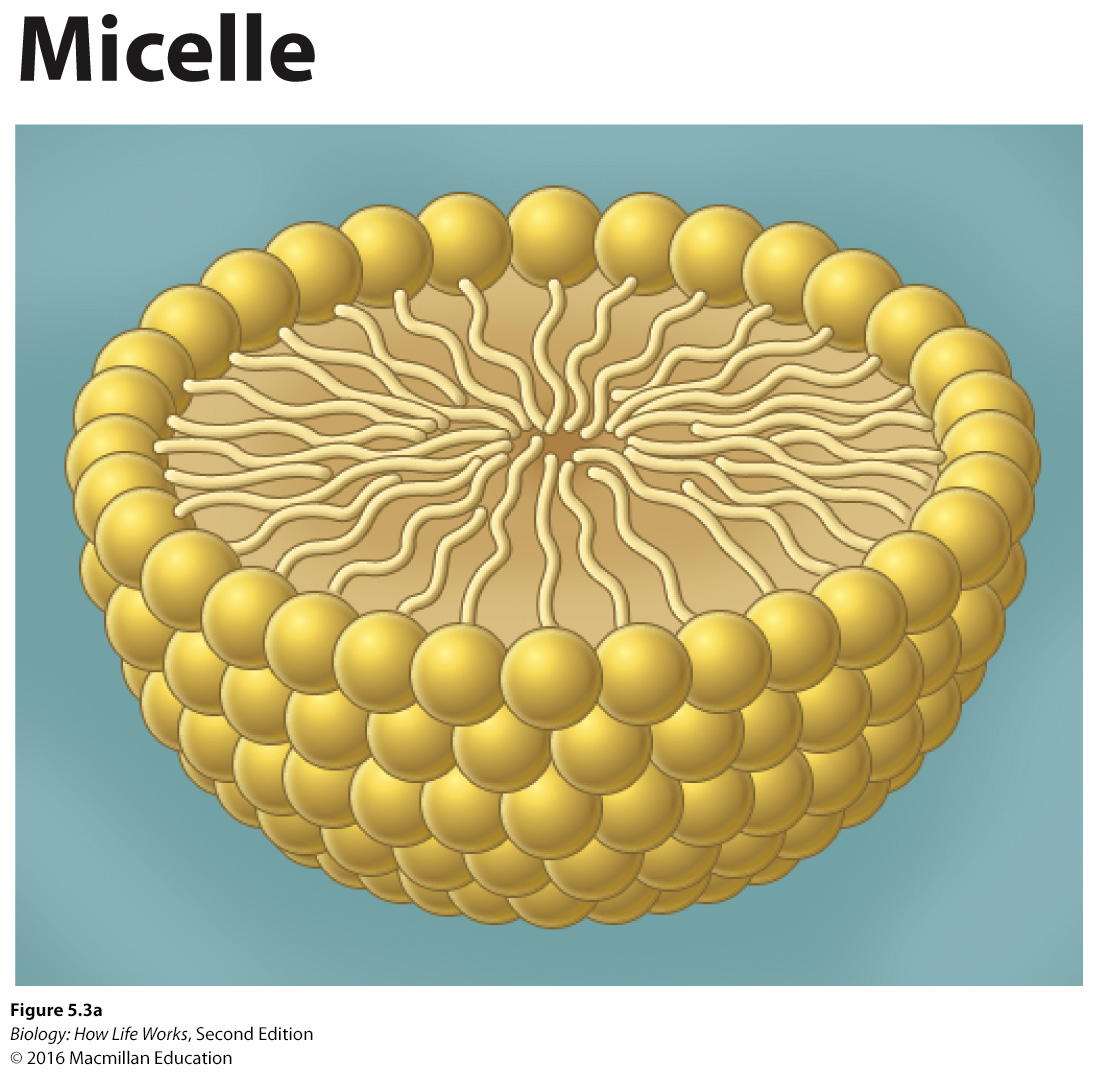
\includegraphics[width=0.6\textwidth]{figures/figure_05_03a.jpg}
	\end{center}
	
\end{frame}


%------------------------------%
% Cellular Membrane VI         %
%------------------------------%
\begin{frame}[t]
\frametitle{Phospholipid Bilayer}
\vspace{0.5cm}

	Plasma membranes are made of a \textbf{\textcolor{myblue}{phospholipid bilayer}}
	
	\vspace{1.0cm}
	
	\begin{columns}
		\begin{column}{0.5\textwidth}
			\centerline{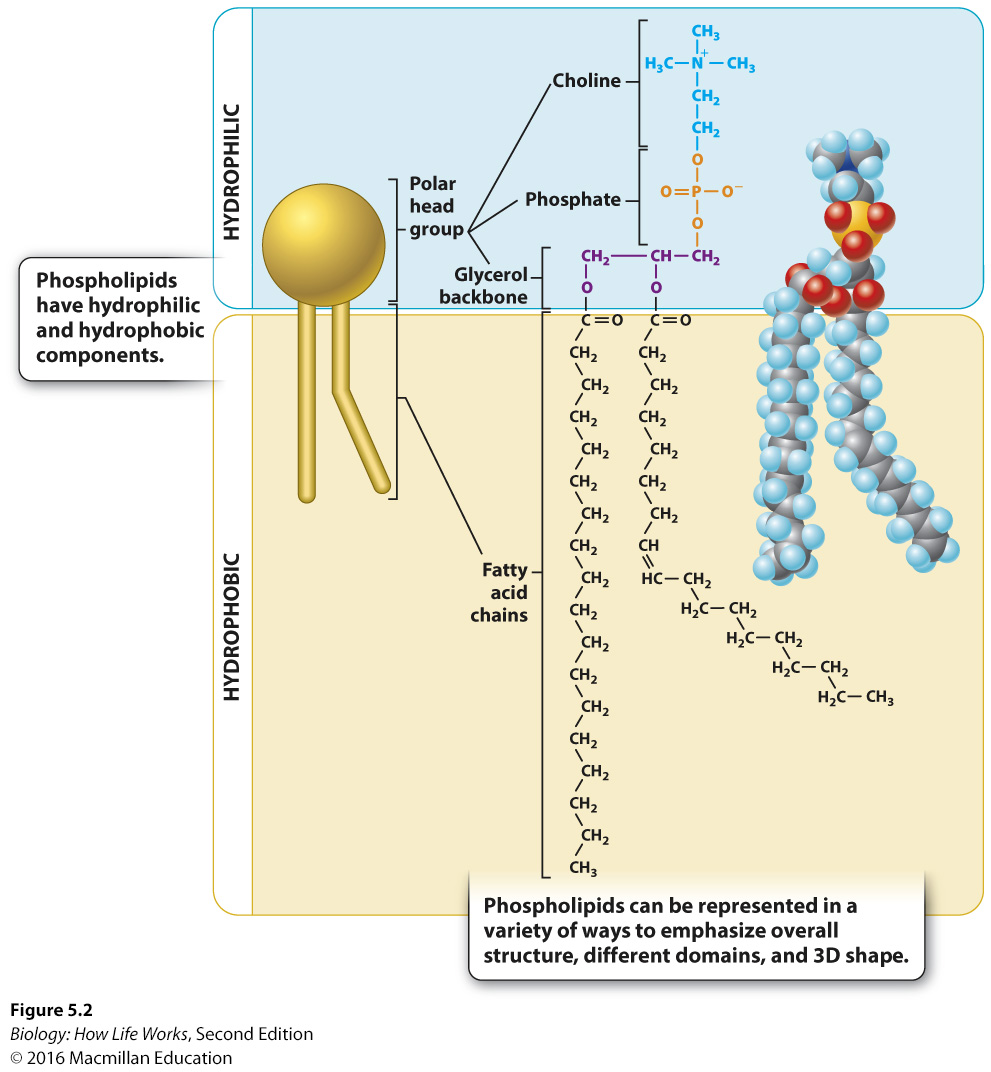
\includegraphics[width=0.9\textwidth]{figures/figure_05_02.jpg}}
		\end{column}
		
		\begin{column}{0.5\textwidth}
			\centerline{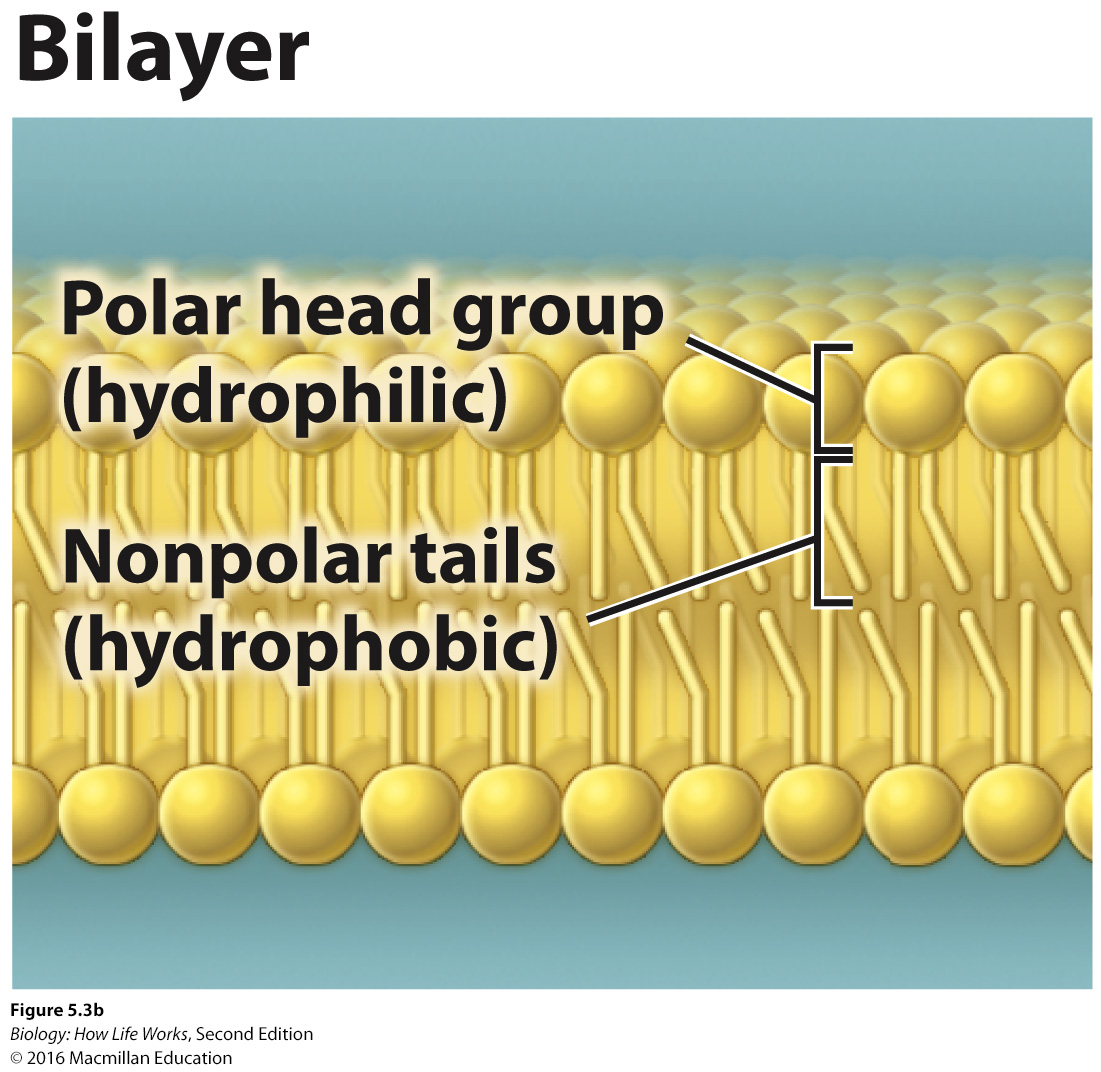
\includegraphics[width=0.8\textwidth]{figures/figure_05_03b.jpg}}
		\end{column}
	\end{columns}	
\end{frame}


%------------------------------%
% Cellular Membrane VII        %
%------------------------------%
\begin{frame}[t]
\frametitle{Phospholipid Bilayer}
\vspace{0.5cm}

	Shape formed in aqueous (water-based) solutions depends on structure\\
	\medskip
	
		\begin{itemize}
			\item Phospholipids with bulky heads and a single hydrophobic tail tend to form micelles
			\medskip
			\item Phospholipids with less bulky head groups and two hydrophobic tails tend to form bilayers
		\end{itemize}	

	\vspace{0.25cm}
	
	\begin{center}
		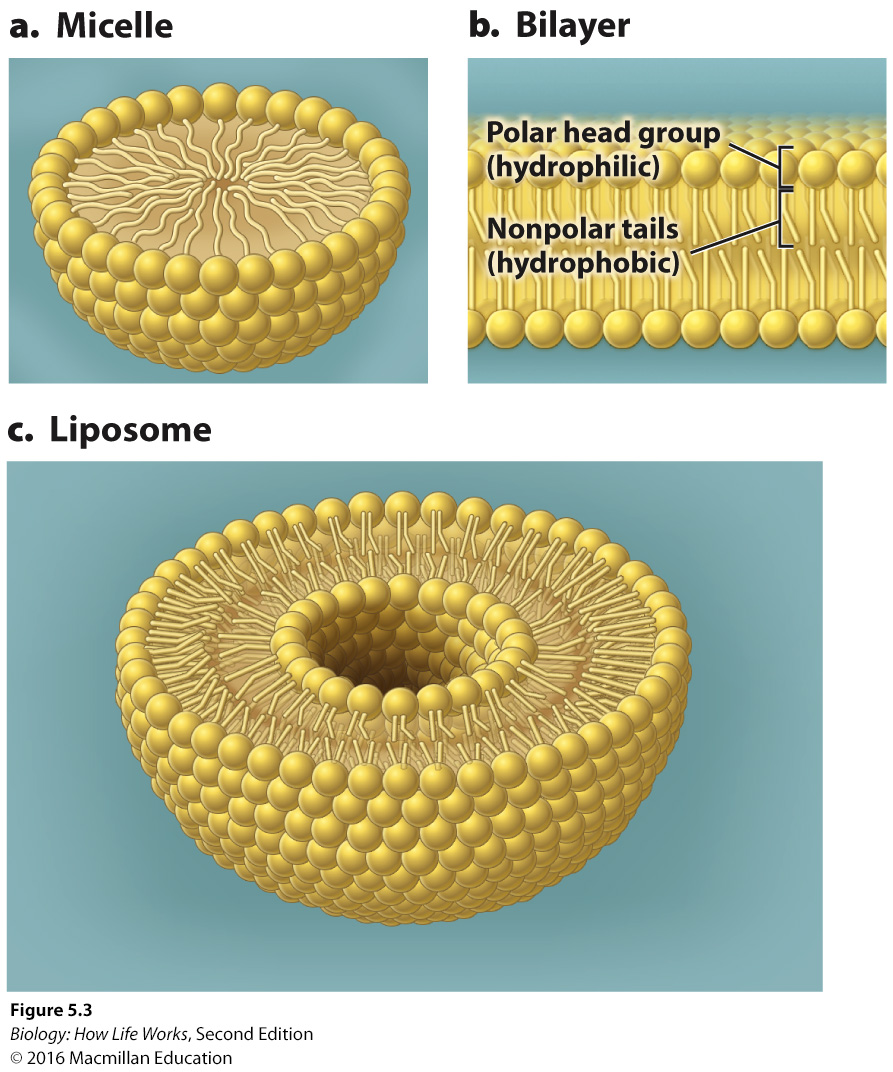
\includegraphics[width=0.3\textwidth]{figures/figure_05_03.jpg}
	\end{center}	
\end{frame}


%------------------------------%
% Cellular Membrane VIII       %
%------------------------------%
\begin{frame}[t]
\frametitle{Phospholipid Bilayer}
\vspace{0.5cm}

	Other important components:
	\medskip
	
		\begin{itemize}
			\item Cholesterol
			\medskip
			\item Proteins
		\end{itemize}	
\end{frame}


%------------------------------%
% Cellular Membrane VIV        %
%------------------------------%
\begin{frame}[t]
\frametitle{Phospholipid Bilayer}
\vspace{0.5cm}

	Other important components:
	\medskip
	
		\begin{itemize}
			\item Cholesterol
			\medskip
			\item \textcolor{gray}{Proteins}
		\end{itemize}	
\end{frame}


%------------------------------%
% Cellular Membrane VV         %
%------------------------------%
\begin{frame}[t]
\frametitle{Phospholipid Bilayer}
\framesubtitle{Cholesterol}
\vspace{0.5cm}

	\begin{columns}
		\begin{column}{0.5\textwidth}
			\begin{center}
				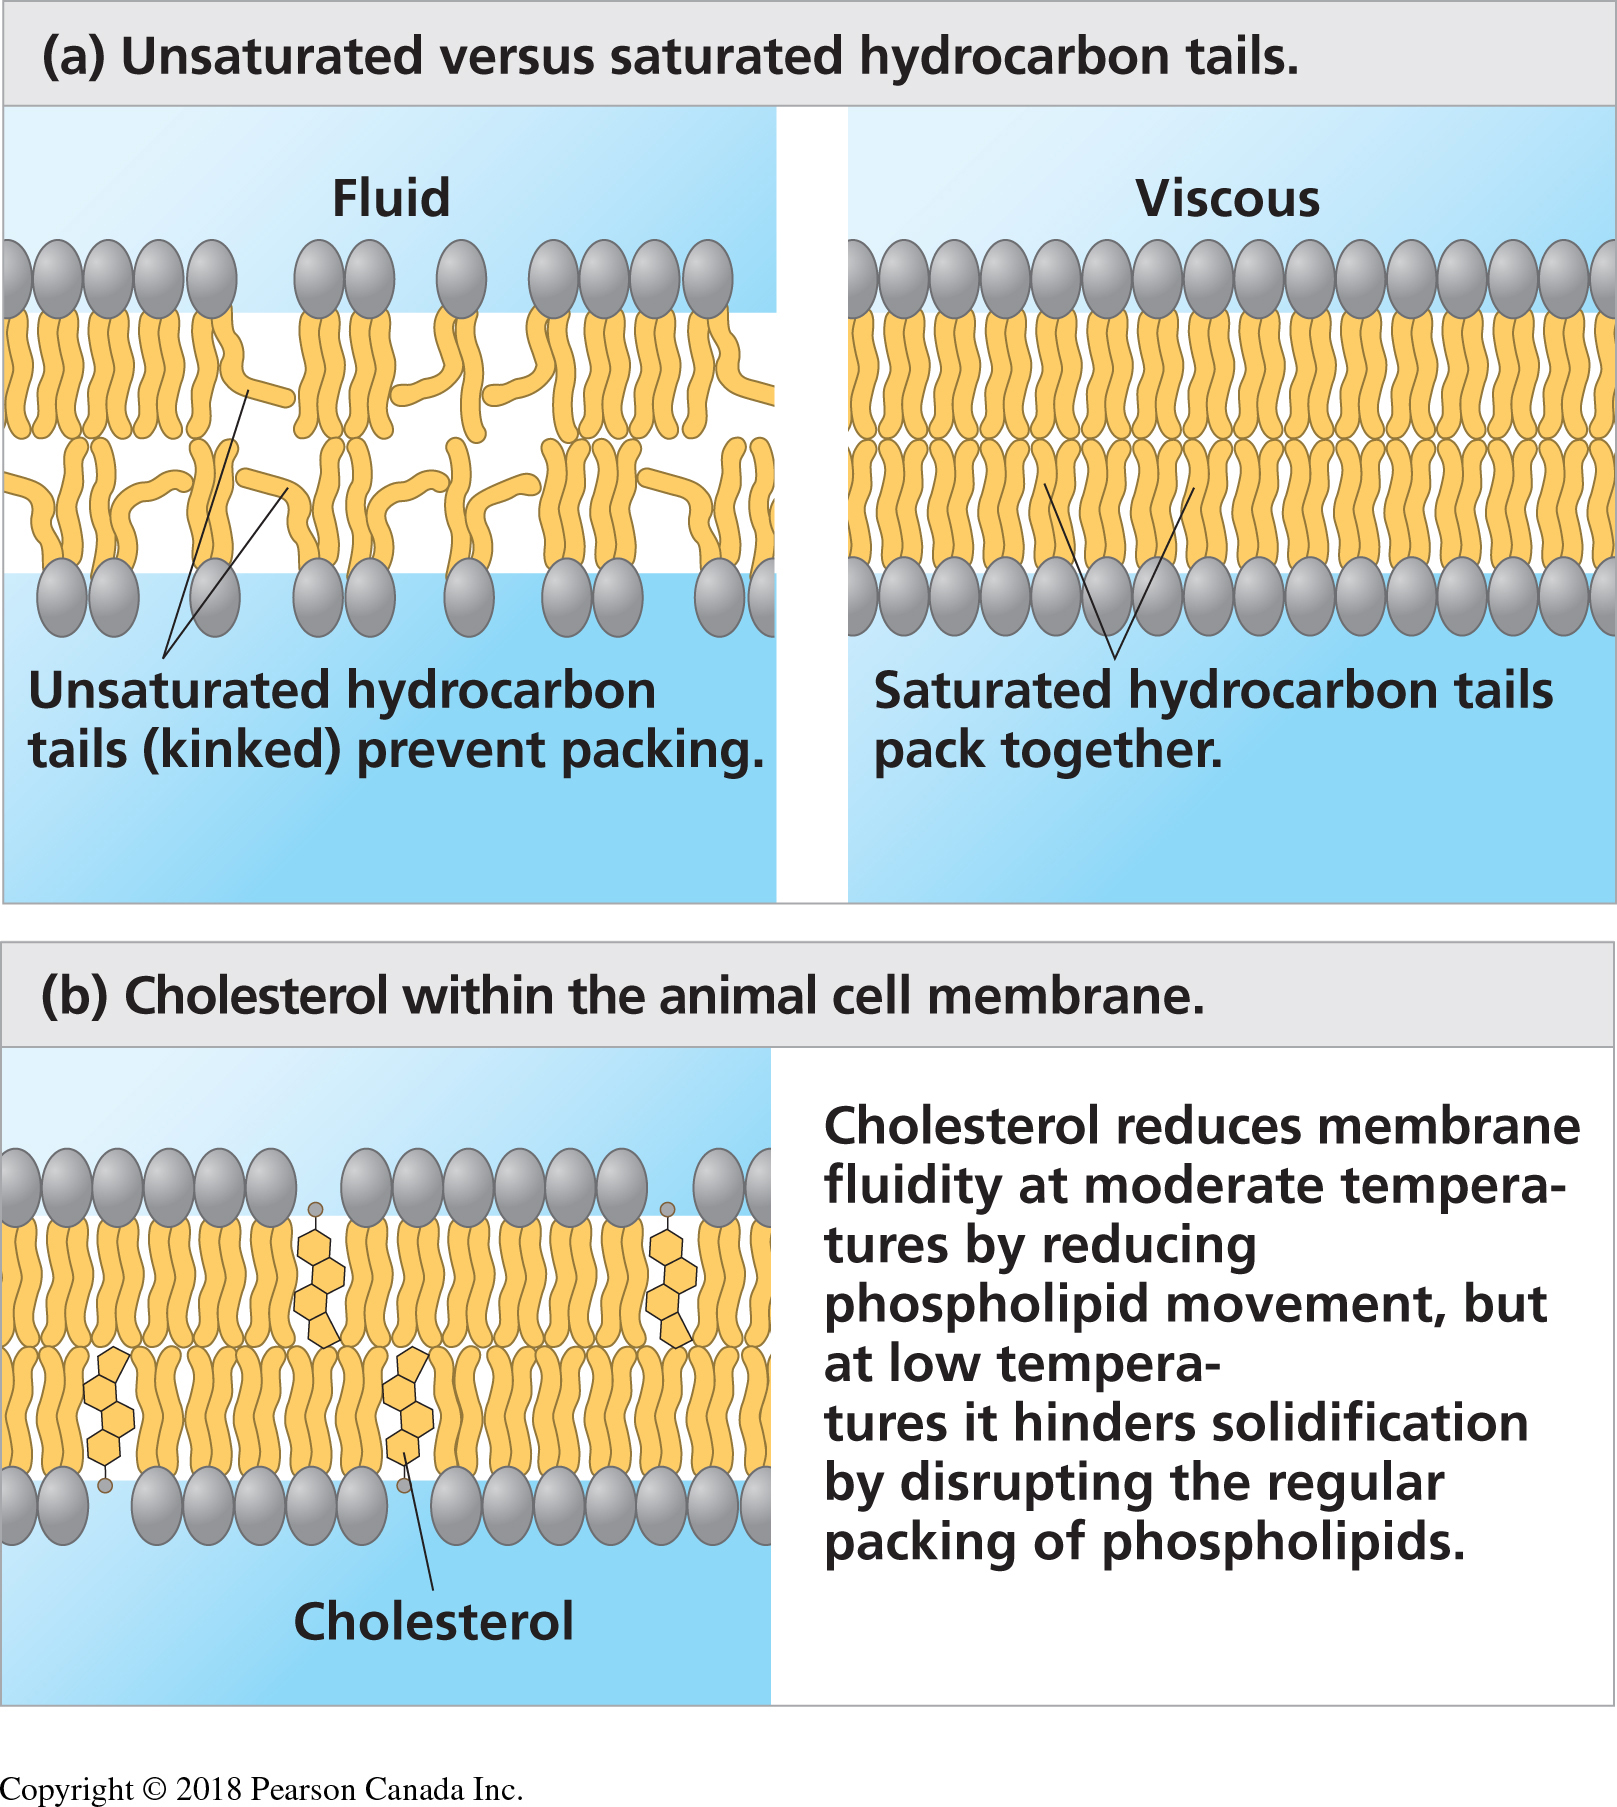
\includegraphics[width=0.7\textwidth]{figures/fg07_05.jpg}
			\end{center}
		\end{column}
		
		\begin{column}{0.5\textwidth}
			\begin{center}
				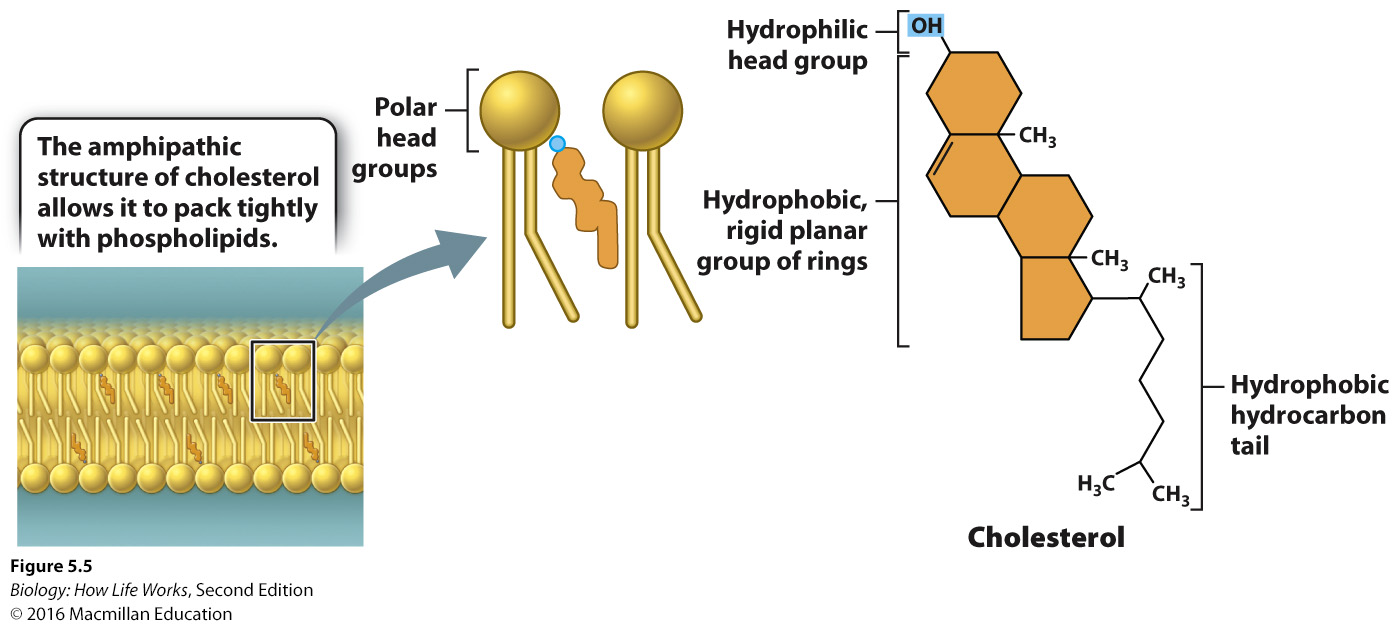
\includegraphics[width=1.0\textwidth]{figures/figure_05_05.jpg}
			\end{center}
		\end{column}
	\end{columns}	
\end{frame}


%------------------------------%
% Cellular Membrane VVI        %
%------------------------------%
\begin{frame}[t]
\frametitle{Phospholipid Bilayer}
\vspace{0.5cm}

	Other important components:
	\medskip
	
		\begin{itemize}
			\item \textcolor{gray}{Cholesterol}
			\medskip
			\item Proteins
		\end{itemize}	
\end{frame}


%------------------------------%
% Cellular Membrane VVII       %
%------------------------------%
\begin{frame}[t]
\frametitle{Phospholipid Bilayer}
\framesubtitle{Proteins}

	\begin{center}
		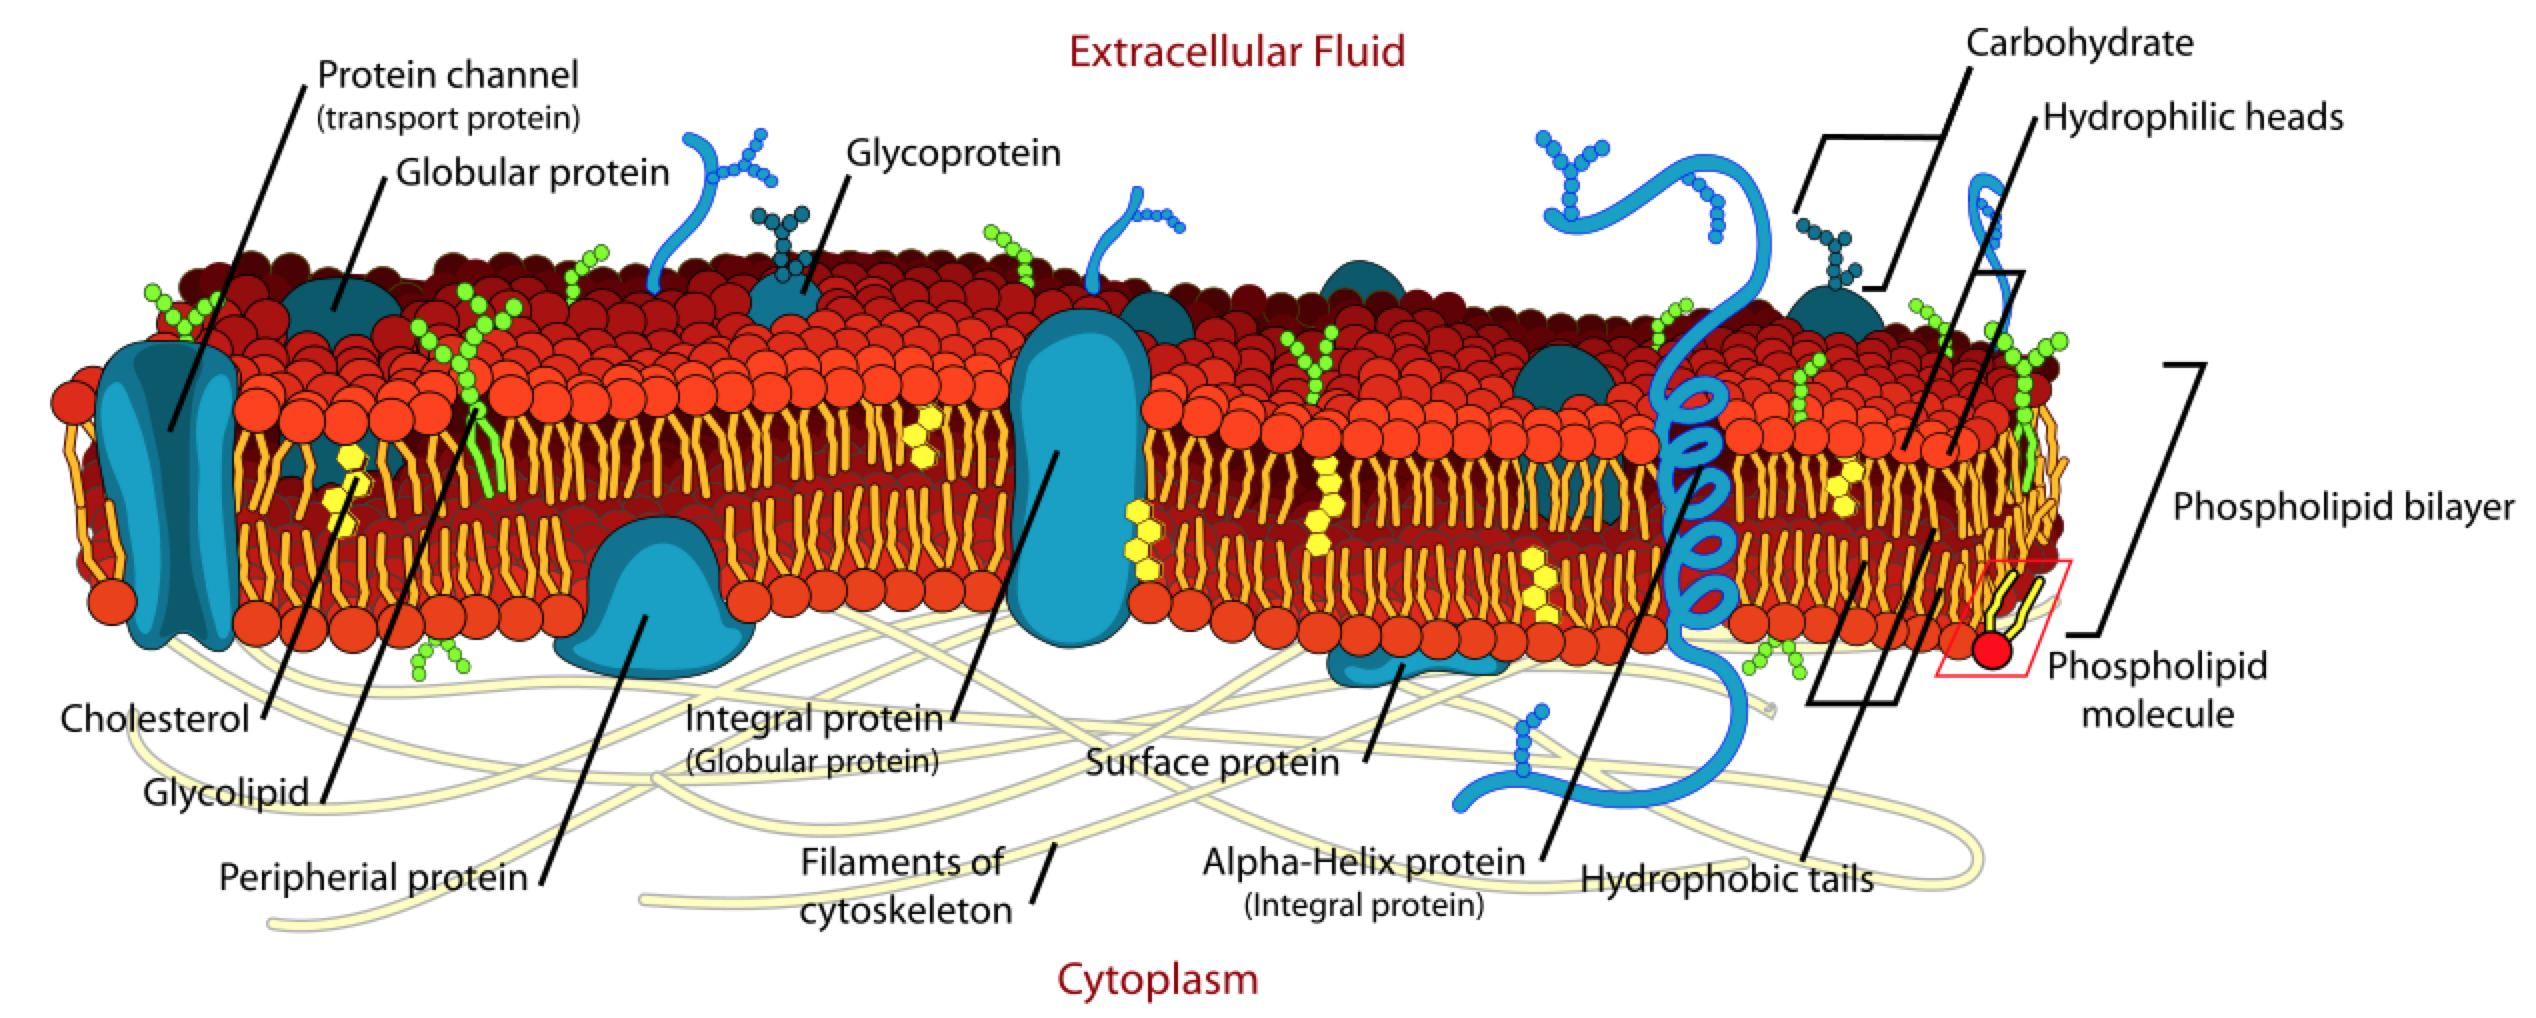
\includegraphics[width=0.7\textwidth]{figures/membraneproteins.png}
	\end{center}

	Cell membranes are full of proteins that serve a number of different roles:\\
	\medskip	
	
		\begin{itemize}
			\item Controlling what is aloud into and out of the cell
			\medskip
			\item Facilitating cellular communation
			\medskip
			\item Allowing cells to evaluate their environment
			\medskip
			\item etc.
		\end{itemize}
	
	\begin{center}
		\textcolor{myblue}{\emph{We will deal with each of these throughout the term}}	
	\end{center}	
\end{frame}


%------------------------------%
% Cellular Membrane VVIII      %
%------------------------------%
\begin{frame}[t]
\frametitle{Phospholipid Bilayer}
\framesubtitle{Proteins}
\vspace{0.5cm}

	Proteins are not static in their position within the membrane\\
	
	\medskip
	
		\begin{itemize}
			\item Move around in a lateral manner
			\medskip
			\item \textcolor{myblue}{``Fluid mosaic model''}
				\begin{itemize}
					\item Membrane is a mosaic of protein molecules bobbing around in the phospholipid bilayer
				\end{itemize}
		\end{itemize}
	
	\vspace{0.25cm}
	
	\begin{center}
		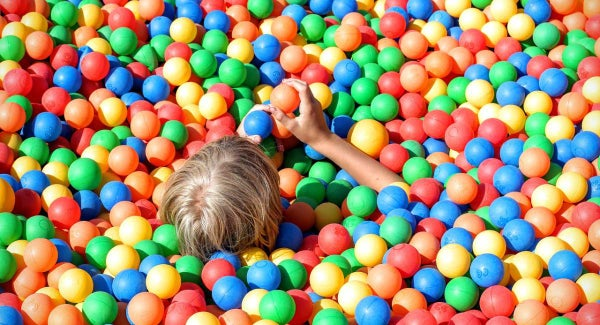
\includegraphics[width=0.5\textwidth]{figures/ballpit.jpg}
	\end{center}	
\end{frame}


%-------------------------------%
% Membrane Transport I          %
%-------------------------------%
\begin{frame}[t]
\frametitle{Cell Membranes Have Selective Permeability}
\vspace{1.0cm}

	\begin{columns}[t]
		\begin{column}{0.5\textwidth}
			\Large{\textbf{\textcolor{myblue2}{Passive Transport}}}\normalsize{}\\
			\medskip
			\textbf{Does not} require energy\\
				\begin{enumerate}
					\item Diffusion/osmosis
					\item Facilitated diffusion
						\begin{enumerate}
							\item Channel proteins
							\item Carrier proteins
						\end{enumerate}
				\end{enumerate}
		\end{column}
		
		\begin{column}{0.5\textwidth}
			\Large{\textbf{\textcolor{myblue2}{Active Transport}}}\normalsize{}\\
			\medskip
			\textbf{Does} require energy\\
		\end{column}
	\end{columns}
\end{frame}


%-------------------------------%
% Membrane Transport Ib         %
%-------------------------------%
\begin{frame}[t]
\frametitle{Cell Membranes Have Selective Permeability}
\vspace{1.0cm}

	\begin{columns}[t]
		\begin{column}{0.5\textwidth}
			\Large{\textbf{\textcolor{myblue2}{Passive Transport}}}\normalsize{}\\
			\medskip
			\textbf{Does not} require energy\\
				\begin{enumerate}
					\item Diffusion/osmosis
					\item \textcolor{gray}{Facilitated diffusion}
						\begin{enumerate}
							\item \textcolor{gray}{Channel proteins}
							\item \textcolor{gray}{Carrier proteins}
						\end{enumerate}
				\end{enumerate}
		\end{column}
		
		\begin{column}{0.5\textwidth}
			\Large{\textbf{\textcolor{gray}{Active Transport}}}\normalsize{}\\
			\medskip
			\textcolor{gray}{\textbf{Does} require energy}\\
		\end{column}
	\end{columns}
\end{frame}


%----------------------------------%
% Membrane Transport II: Diffusion %
%----------------------------------%
\begin{frame}[t]
\frametitle{Passive Transport}
\framesubtitle{Diffusion}
\vspace{0.5cm}

	When the concentration of molecules differs in different locations, they will move to equalize their concentration: ``\emph{Move down their concentration gradient}''\\

	\vspace{0.5cm}
	
	Reach a \textcolor{myblue}{dynamic equilibrium}: molecules still moving, but relative [ ] remains the same	
	
	\vspace{0.5cm}
	
	\begin{center}
		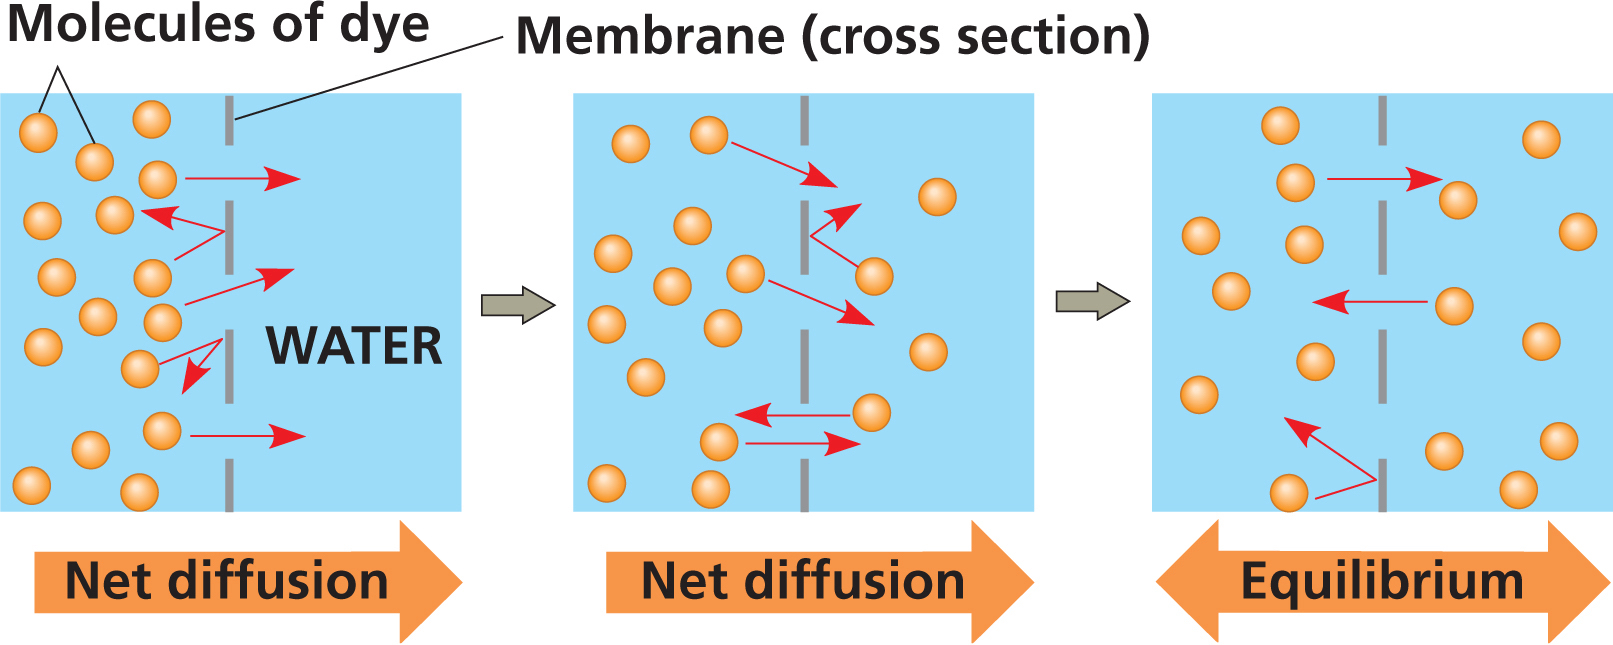
\includegraphics[width=0.8\textwidth]{figures/fg07_10a.jpg}
	\end{center}
\end{frame}


%-----------------------------------%
% Membrane Transport III: Diffusion %
%-----------------------------------%
\begin{frame}[t]
\frametitle{Passive Transport}
\framesubtitle{Diffusion}
\vspace{0.5cm}

	Equilibrium is independent for each molecule type (not overall!)
	
	\vspace{0.5cm}
	
	\begin{center}
		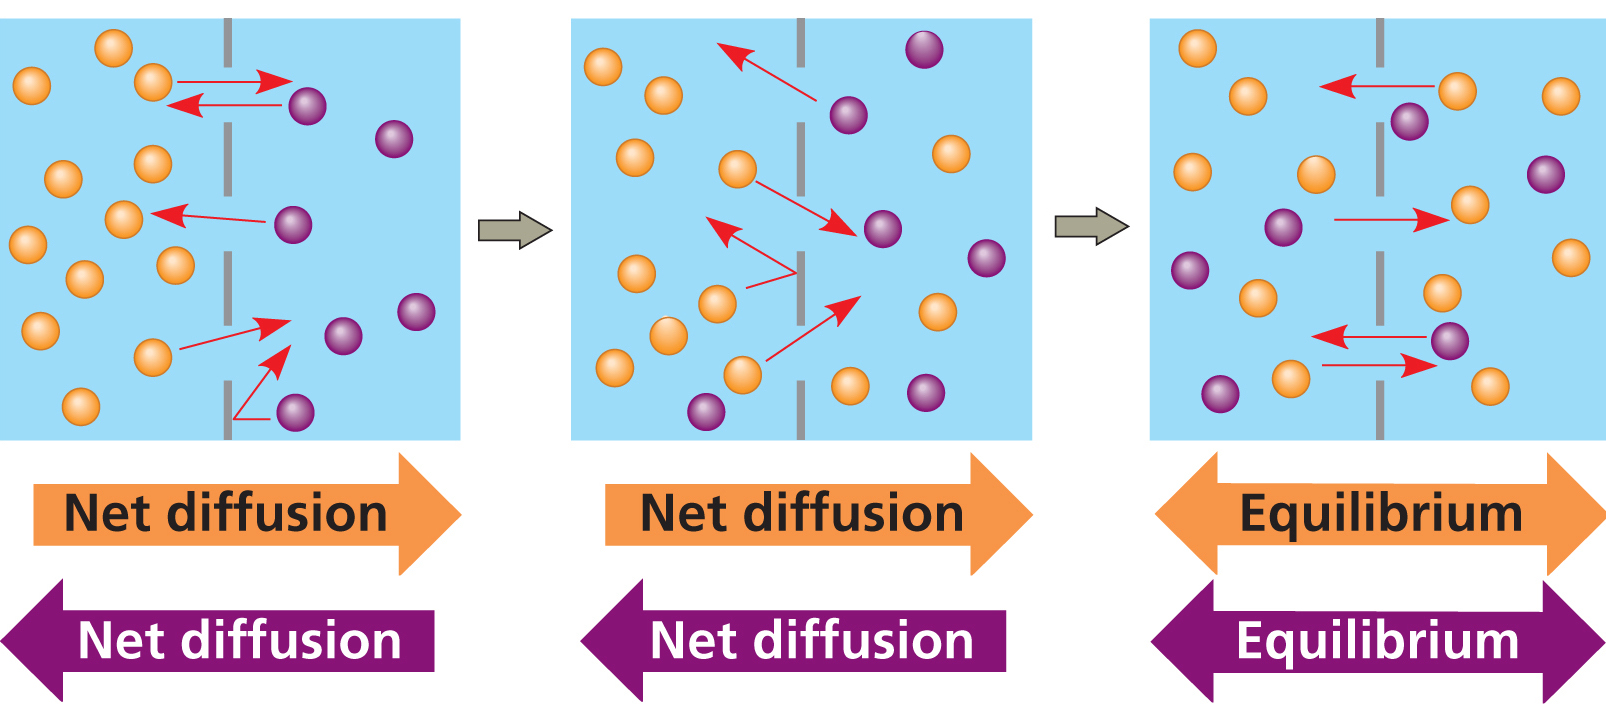
\includegraphics[width=0.8\textwidth]{figures/fg07_10b.jpg}
	\end{center}
\end{frame}


%----------------------------------%
% Membrane Transport IV: Diffusion %
%----------------------------------%
\begin{frame}[t]
\frametitle{Passive Transport}
\framesubtitle{Diffusion}
\vspace{0.5cm}

	Small non-polar (hydrophobic) molecules can diffuse across the membrane
		\medskip
		\begin{itemize}
			\item O$_{2}$
			\medskip
			\item CO$_{2}$
		\end{itemize}
\end{frame}


%----------------------------------%
% Membrane Transport V: Diffusion  %
%----------------------------------%
\begin{frame}
\frametitle{Passive Transport}
\framesubtitle{Diffusion}

	\begin{center}
		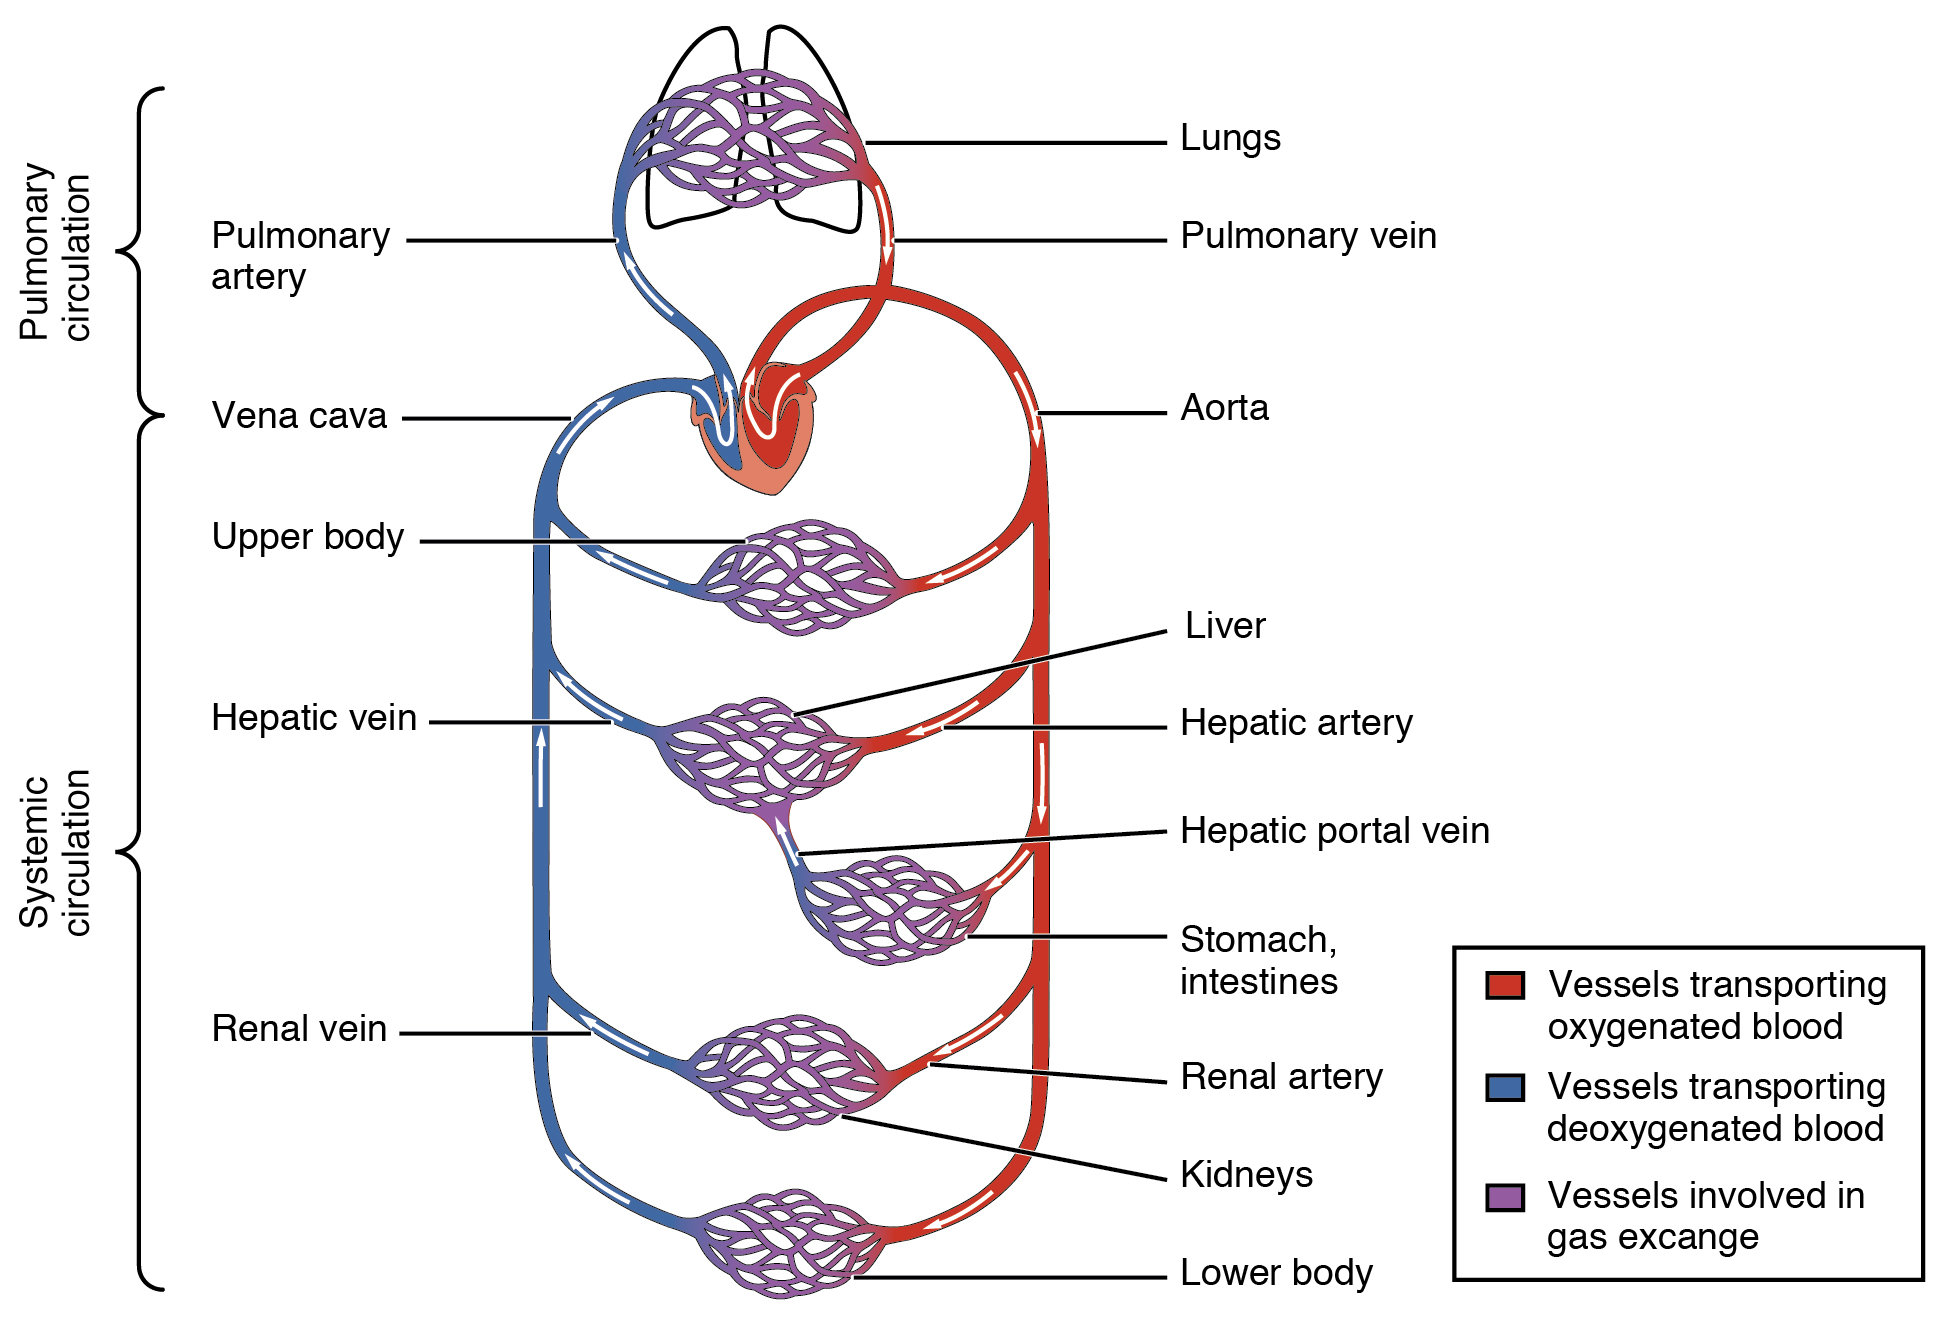
\includegraphics[width=0.75\textwidth]{figures/circulation.jpg}
	\end{center}	
\end{frame}


%----------------------------------%
% Membrane Transport VI: Osmosis   %
%----------------------------------%
\begin{frame}[t]
\frametitle{Passive Transport}
\framesubtitle{Osmosis}

	When the diffusing molecule is water
		\medskip
		\begin{itemize}
			\item Water mostly passes through specialized channels (not diffusion)
			\medskip
			\item Concept is similar to diffusion
		\end{itemize}
	
		\begin{center}
			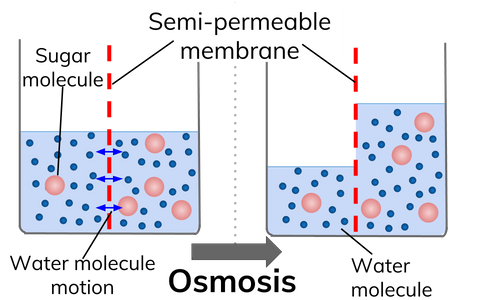
\includegraphics[width=0.6\textwidth]{figures/osmosis.png}
		\end{center}	
\end{frame}


%----------------------------------%
% Membrane Transport VII: Osmosis  %
%----------------------------------%
\begin{frame}[t]
\frametitle{Passive Transport}
\framesubtitle{Osmosis}

	\begin{center}
		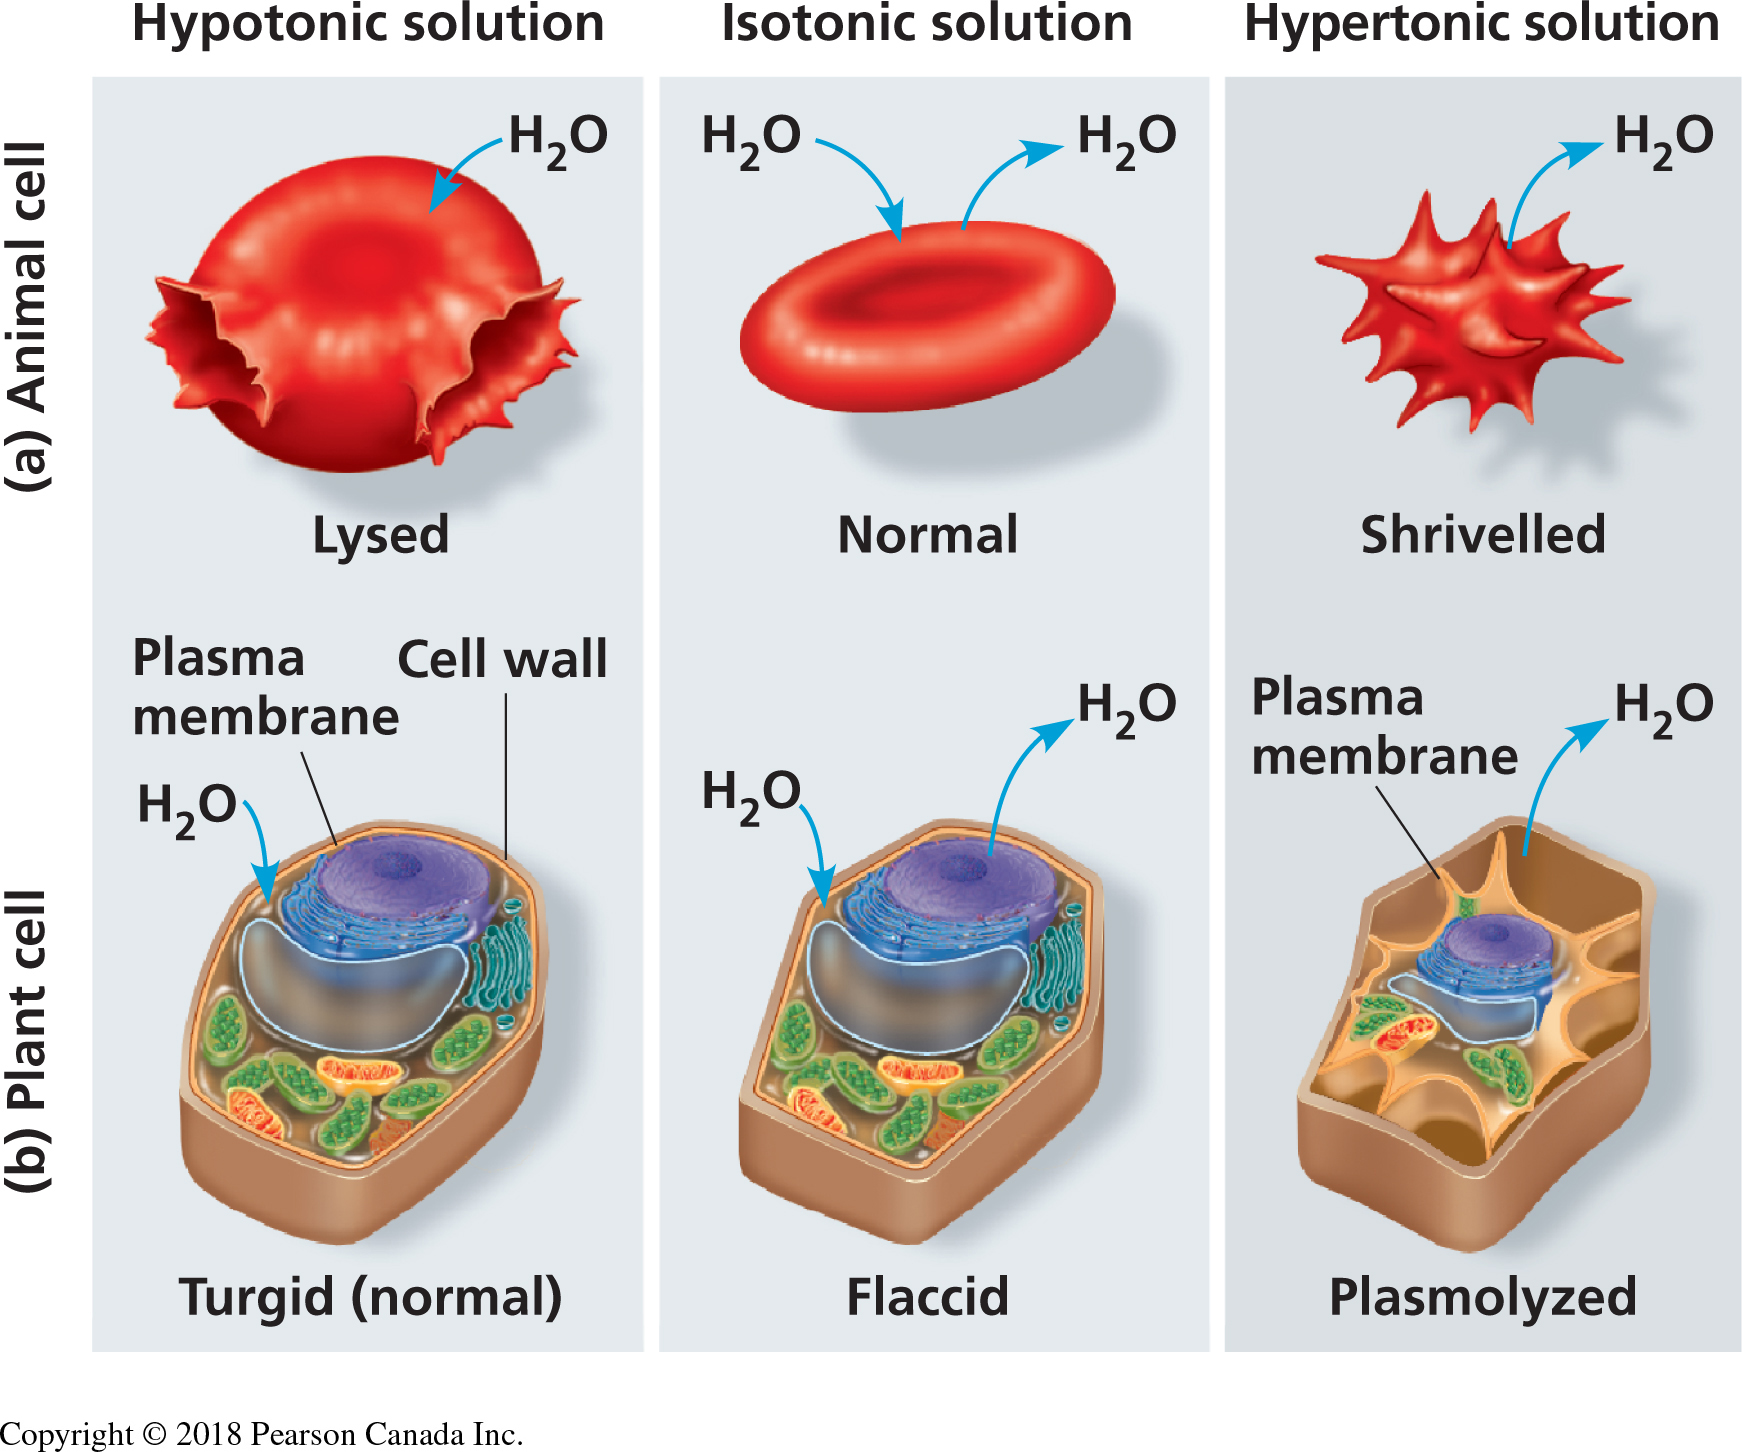
\includegraphics[width=0.75\textwidth]{figures/fg07_12.jpg}
	\end{center}	
\end{frame}


%----------------------------------%
% Membrane Transport VIII: Osmosis %
%----------------------------------%
\begin{frame}[t]
\frametitle{Passive Transport}
\framesubtitle{Osmosis}
\vspace{0.5cm}

	\begin{columns}
		\begin{column}{0.5\textwidth}
			\begin{center}
				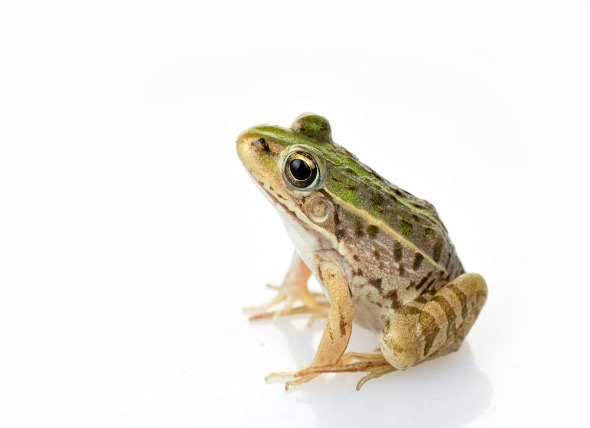
\includegraphics[width=0.9\textwidth]{figures/frog.jpg}
			\end{center}
		\end{column}
		
		\begin{column}{0.5\textwidth}
			\begin{center}
				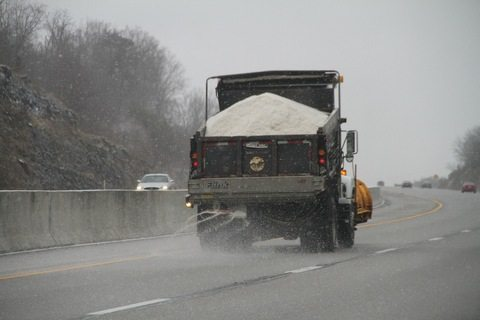
\includegraphics[width=0.9\textwidth]{figures/saltingroad.jpg}
			\end{center}
		\end{column}
	\end{columns}	
\end{frame}


%------------------------------------------%
% Membrane Transport IX:  Channel proteins %
%------------------------------------------%
\begin{frame}[t]
\frametitle{Passive Transport}
\vspace{1.0cm}

	\begin{columns}[t]
		\begin{column}{0.5\textwidth}
			\Large{\textbf{\textcolor{myblue2}{Passive Transport}}}\normalsize{}\\
			\medskip
			\textbf{Does not} require energy\\
				\begin{enumerate}
					\item \textcolor{gray}{Diffusion/osmosis}
					\item Facilitated diffusion
						\begin{enumerate}
							\item Channel proteins
							\item Carrier proteins
						\end{enumerate}
				\end{enumerate}
		\end{column}
		
		\begin{column}{0.5\textwidth}
			\Large{\textbf{\textcolor{gray}{Active Transport}}}\normalsize{}\\
			\medskip
			\textcolor{gray}{\textbf{Does} require energy}\\
		\end{column}
	\end{columns}
\end{frame}


%-----------------------------------------%
% Membrane Transport X:  Channel proteins %
%-----------------------------------------%
\begin{frame}[t]
\frametitle{Passive Transport}
\framesubtitle{Facilitated Diffusion 1 - Channel Proteins}
\vspace{0.5cm}

	Just provide a ``safe'' passageway through which molecules can pass
		\begin{itemize}
			\item Usually specialized for a particular molecule or type of molecules
			\item \textcolor{myblue}{Aquaporins} for water
		\end{itemize}

	\vspace{0.5cm}
	
	\begin{center}
		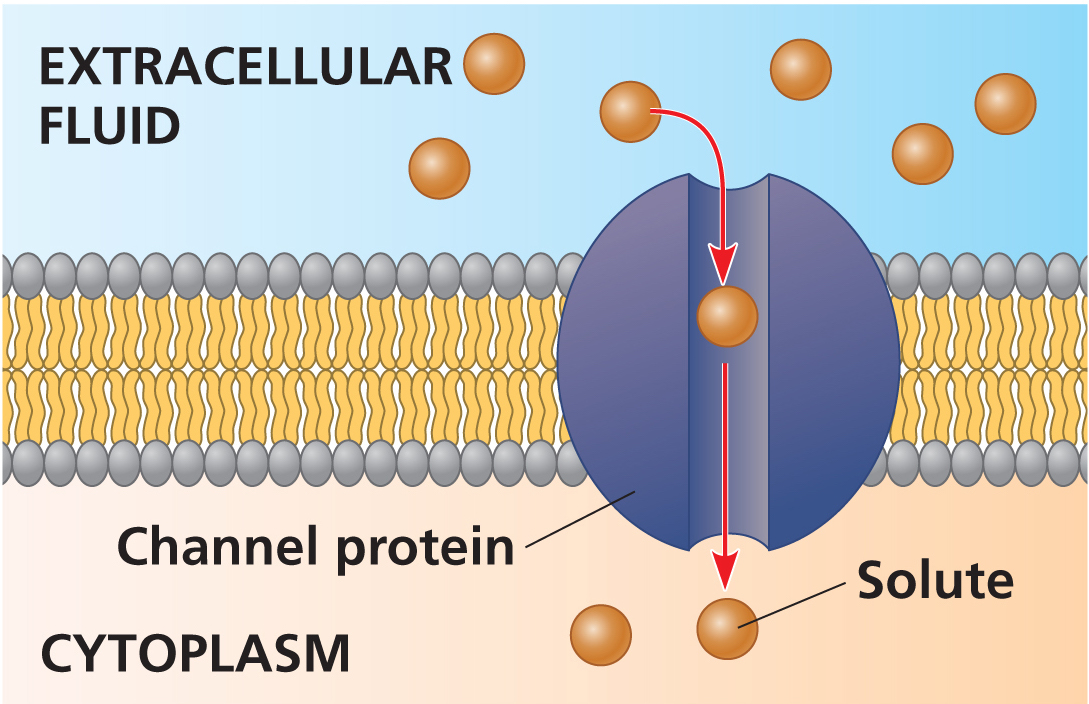
\includegraphics[width=0.45\textwidth]{figures/fg07_14a.jpg}
	\end{center}
\end{frame}


%------------------------------------------%
% Membrane Transport XI:  Carrier proteins %
%------------------------------------------%
\begin{frame}[t]
\frametitle{Passive Transport}
\framesubtitle{Facilitated Diffusion 2 - Carrier Proteins}
\vspace{0.5cm}

	Undergo a change in shape when bound to molecules that facilitates their passage through the membrane

	\vspace{0.5cm}
	
	\begin{center}
		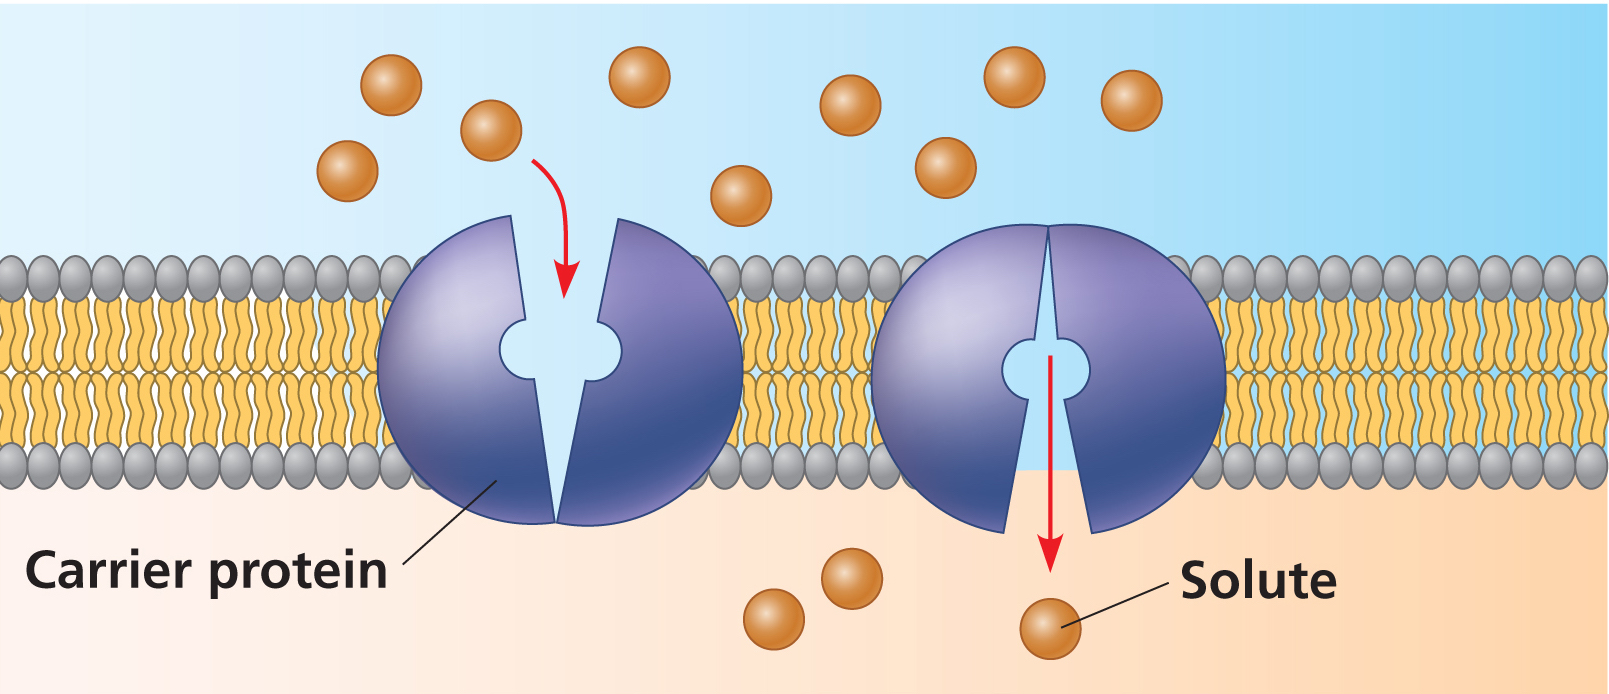
\includegraphics[width=0.65\textwidth]{figures/fg07_14b.jpg}
	\end{center}
\end{frame}


%--------------------------------------------%
% Membrane Transport XV:  Active Transport  %
%--------------------------------------------%
\begin{frame}
\frametitle{Passive Transport}
\framesubtitle{Facilitated Diffusion 2 - Carrier Proteins}
\vspace{0.5cm}

	\begin{center}
		\href{https://www.youtube.com/watch?v=IX-kLh34KcQ}{\LARGE{\textbf{Video}}}
	\end{center}

\end{frame}


%-------------------------------------------%
% Membrane Transport XII: Passive Transport %
%-------------------------------------------%
\begin{frame}[t]
\frametitle{Passive Transport}
\vspace{1.0cm}

	\begin{columns}[t]
		\begin{column}{0.5\textwidth}
			\Large{\textbf{\textcolor{myblue2}{Passive Transport}}}\normalsize{}\\
			\medskip
			\textbf{Does not} require energy\\
				\begin{enumerate}
					\item Diffusion/osmosis
					\item Facilitated diffusion
						\begin{enumerate}
							\item Channel proteins
							\item Carrier proteins
						\end{enumerate}
				\end{enumerate}
		\end{column}
		
		\begin{column}{0.5\textwidth}
			\Large{\textbf{\textcolor{gray}{Active Transport}}}\normalsize{}\\
			\medskip
			\textcolor{gray}{\textbf{Does} require energy}\\
		\end{column}
	\end{columns}
	
	\vspace{1.0cm} 
	
	All involve molecules moving down their concentration gradient.
\end{frame}


%-------------------------------------------%
% Membrane Transport XII: Passive Transport %
%-------------------------------------------%
\begin{frame}
\frametitle{Passive Transport}

	\begin{center}
		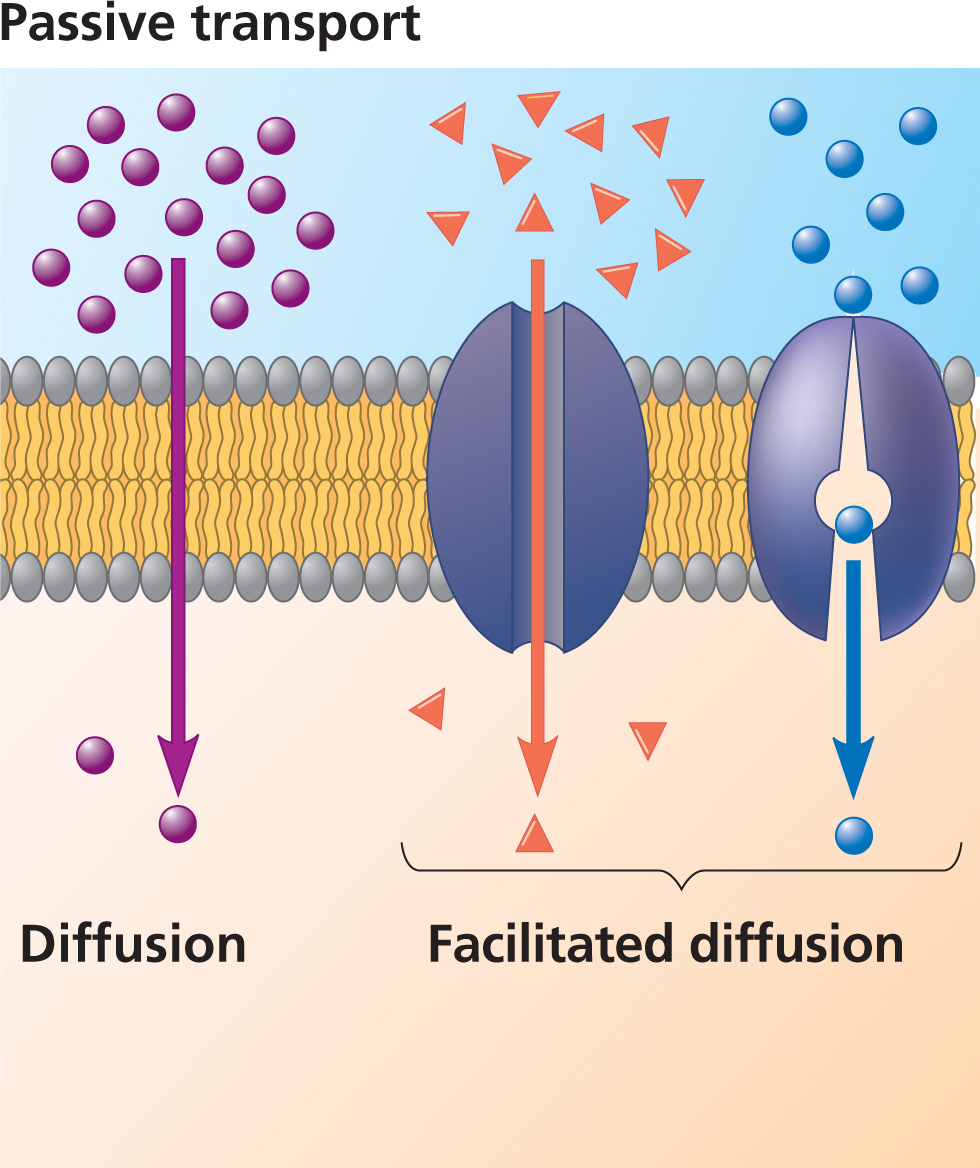
\includegraphics[width=0.55\textwidth]{figures/fg07_16a.jpg}
	\end{center}
\end{frame}



%--------------------------------------------%
% Membrane Transport XIII: Active Transport  %
%--------------------------------------------%
\begin{frame}[t]
\frametitle{Active Transport}
\vspace{1.0cm}

	\begin{columns}[t]
		\begin{column}{0.5\textwidth}
			\Large{\textbf{\textcolor{gray}{Passive Transport}}}\normalsize{}\\
			\medskip
			\textcolor{gray}{\textbf{Does not} require energy}\\
				\begin{enumerate}
					\item \textcolor{gray}{Diffusion/osmosis}
					\item \textcolor{gray}{Facilitated diffusion}
						\begin{enumerate}
							\item \textcolor{gray}{Channel proteins}
							\item \textcolor{gray}{Carrier proteins}
						\end{enumerate}
				\end{enumerate}
		\end{column}
		
		\begin{column}{0.5\textwidth}
			\Large{\textbf{\textcolor{myblue}{Active Transport}}}\normalsize{}\\
			\medskip
			\textbf{Does} require energy
		\end{column}
	\end{columns}
\end{frame}


%--------------------------------------------%
% Membrane Transport XIV:  Active Transport  %
%--------------------------------------------%
\begin{frame}[t]
\frametitle{Active Transport}
\vspace{0.5cm}

	Moves molecules \textbf{against} their concentration gradient
		\begin{itemize}
			\item Requires energy! (usually in the form of ATP)
			\item Extremely important: Allows cells to maintain internal conditions that are \emph{different} from the external environment
		\end{itemize}

	\begin{center}
		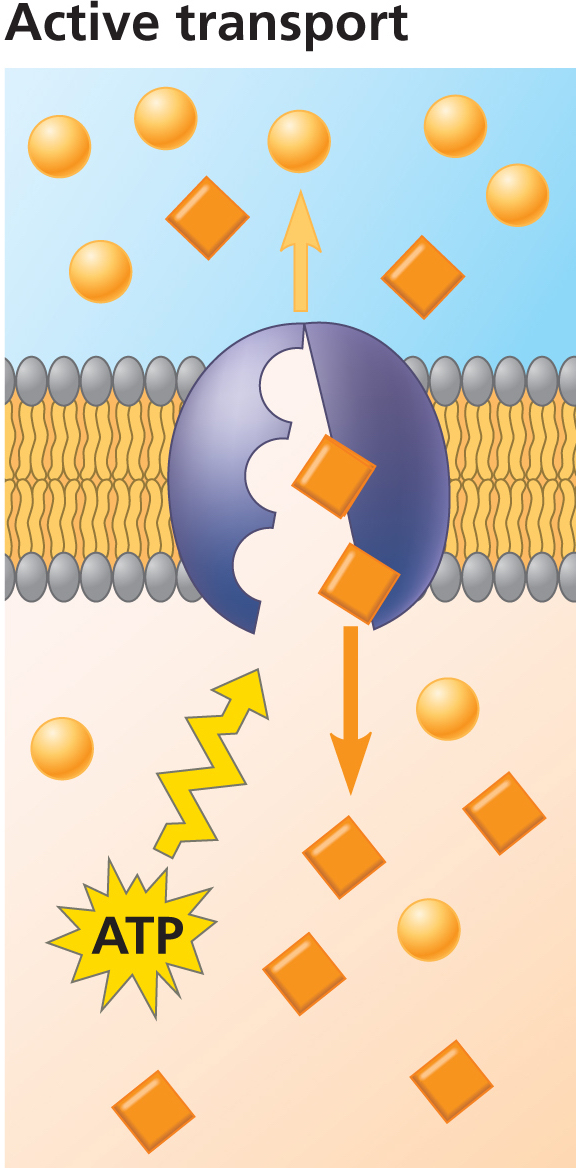
\includegraphics[width=0.20\textwidth]{figures/fg07_16b.jpg}
	\end{center}
\end{frame}


%--------------------------------------------%
% Membrane Transport XV:  Active Transport  %
%--------------------------------------------%
\begin{frame}
\frametitle{Active Transport}
\vspace{0.5cm}

	\begin{center}
		\href{https://www.youtube.com/watch?v=M6_NCdV7YO8}{\LARGE{\textbf{Video}}}
	\end{center}

\end{frame}


%--------------------------------------------%
% Membrane Transport XVI:  Active Transport  %
%--------------------------------------------%
\begin{frame}
\frametitle{Selective Permeability}
\vspace{0.5cm}

	\begin{center}
		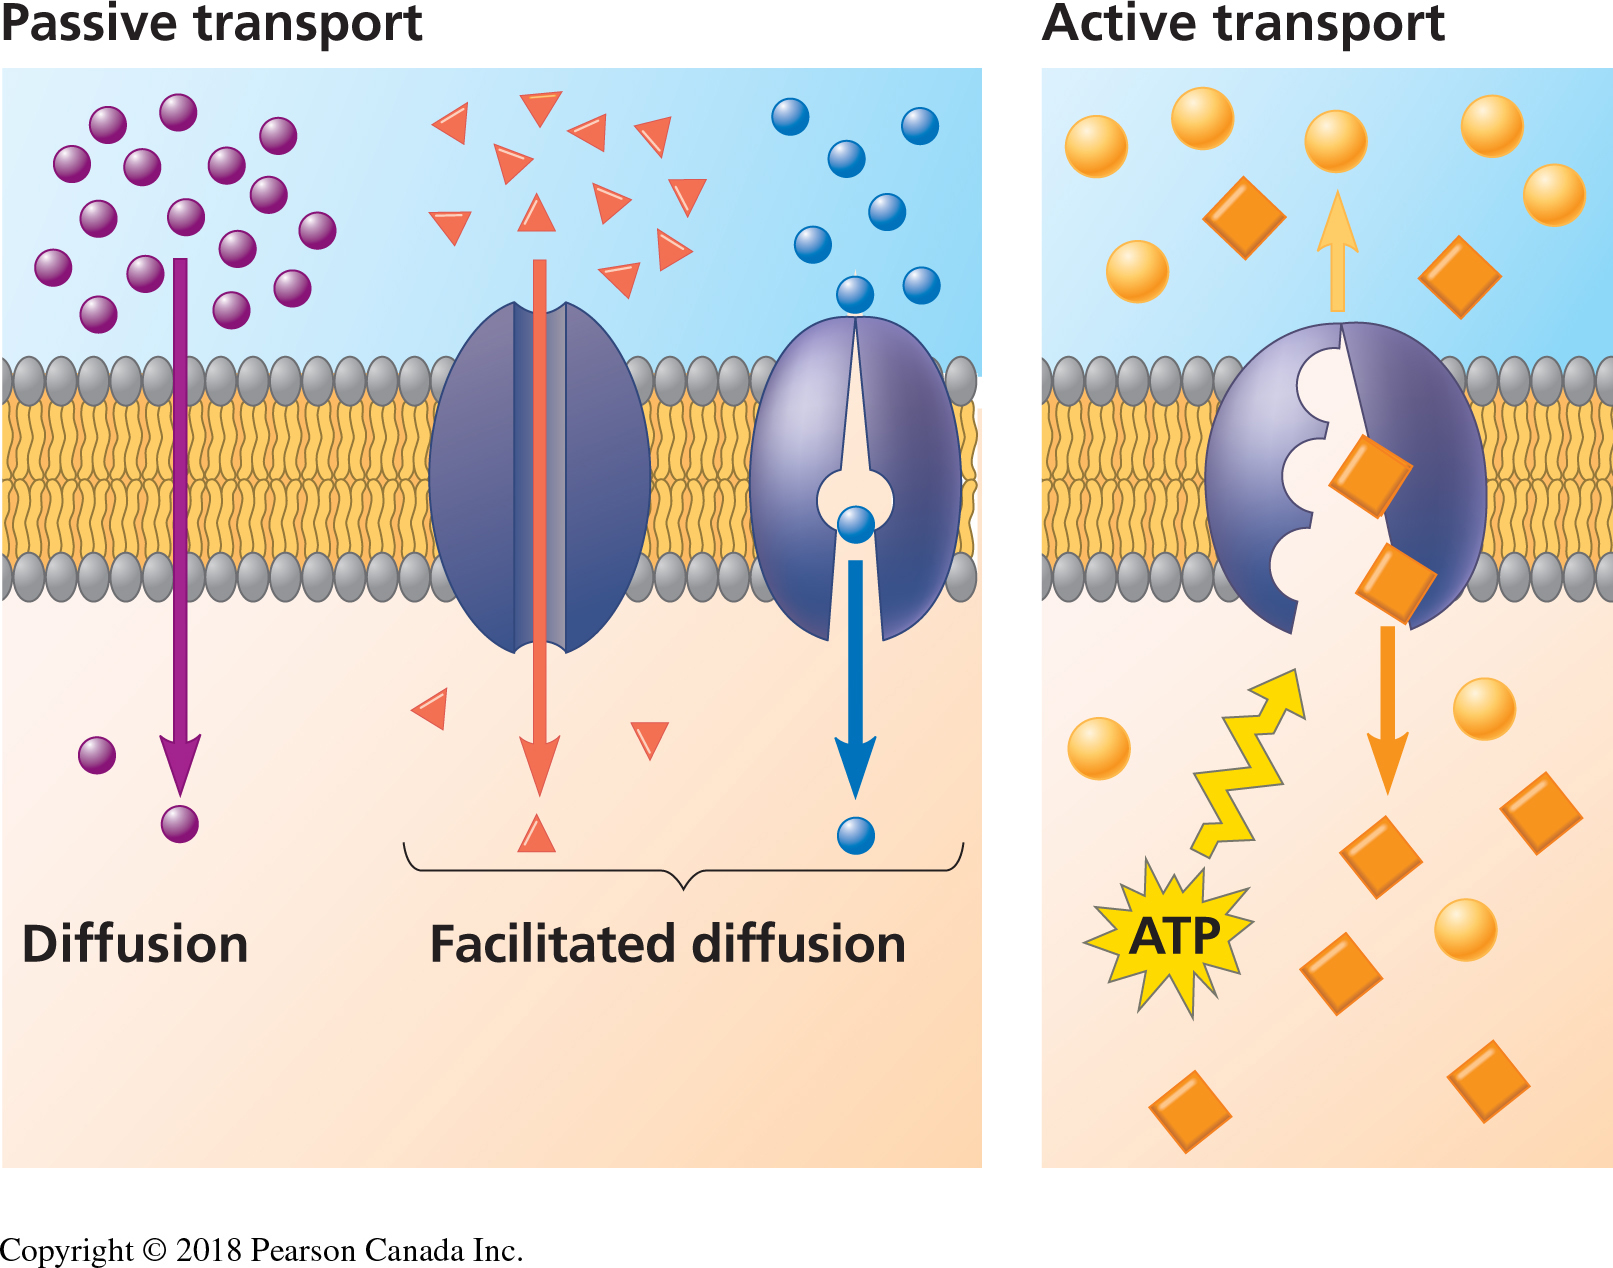
\includegraphics[width=0.70\textwidth]{figures/fg07_16.jpg}
	\end{center}

\end{frame}


%-----------------------------------%
% Internal Components of the Cell   %
%-----------------------------------%
\begin{frame}
	
	\begin{center}
		\LARGE{\textcolor{myblue}{Internal Components of the Cell}}
	\end{center}

\end{frame}


%-------------------------------%
% Prokaryotes & Eukaryotes I    %
%-------------------------------%
\begin{frame}[t]

	\begin{center}
		\textcolor{myblue}{Are two main types of cells: \textbf{prokaryotic} cells and \textbf{eukaryotic} cells}\\
		
		\vspace{1.0cm}
		
		\begin{tabular}{p{3.0cm} p{3.0cm} p{3.5cm}}
			\textbf{Characteristic} & \textbf{Prokaryotes} & \textbf{Eukaryotes}\\
			\midrule
			Size & \texttt{small (1-5$\mu$m)} & \texttt{larger (10-100$\mu$m)}\\
			\addlinespace
			\addlinespace
			Nucleus & \texttt{No} & \texttt{Yes}\\
			\addlinespace
			\addlinespace
			Membrane-bound organelles & \texttt{No} & \texttt{Yes}\\
			\addlinespace
			\addlinespace
			DNA & \texttt{single, circular chromosome} & \texttt{paired chromosomes, often many}\\
			\addlinespace
			\addlinespace
			etc. & &\\
		\end{tabular}
	\end{center}
\end{frame}


%-------------------------------%
% Prokaryotes & Eukaryotes II   %
%-------------------------------%
\begin{frame}
	\begin{columns}
		\begin{column}{0.5\textwidth}
			\begin{center}
				\textbf{Prokaryotic Cell}\\
				\vspace{0.5cm}
				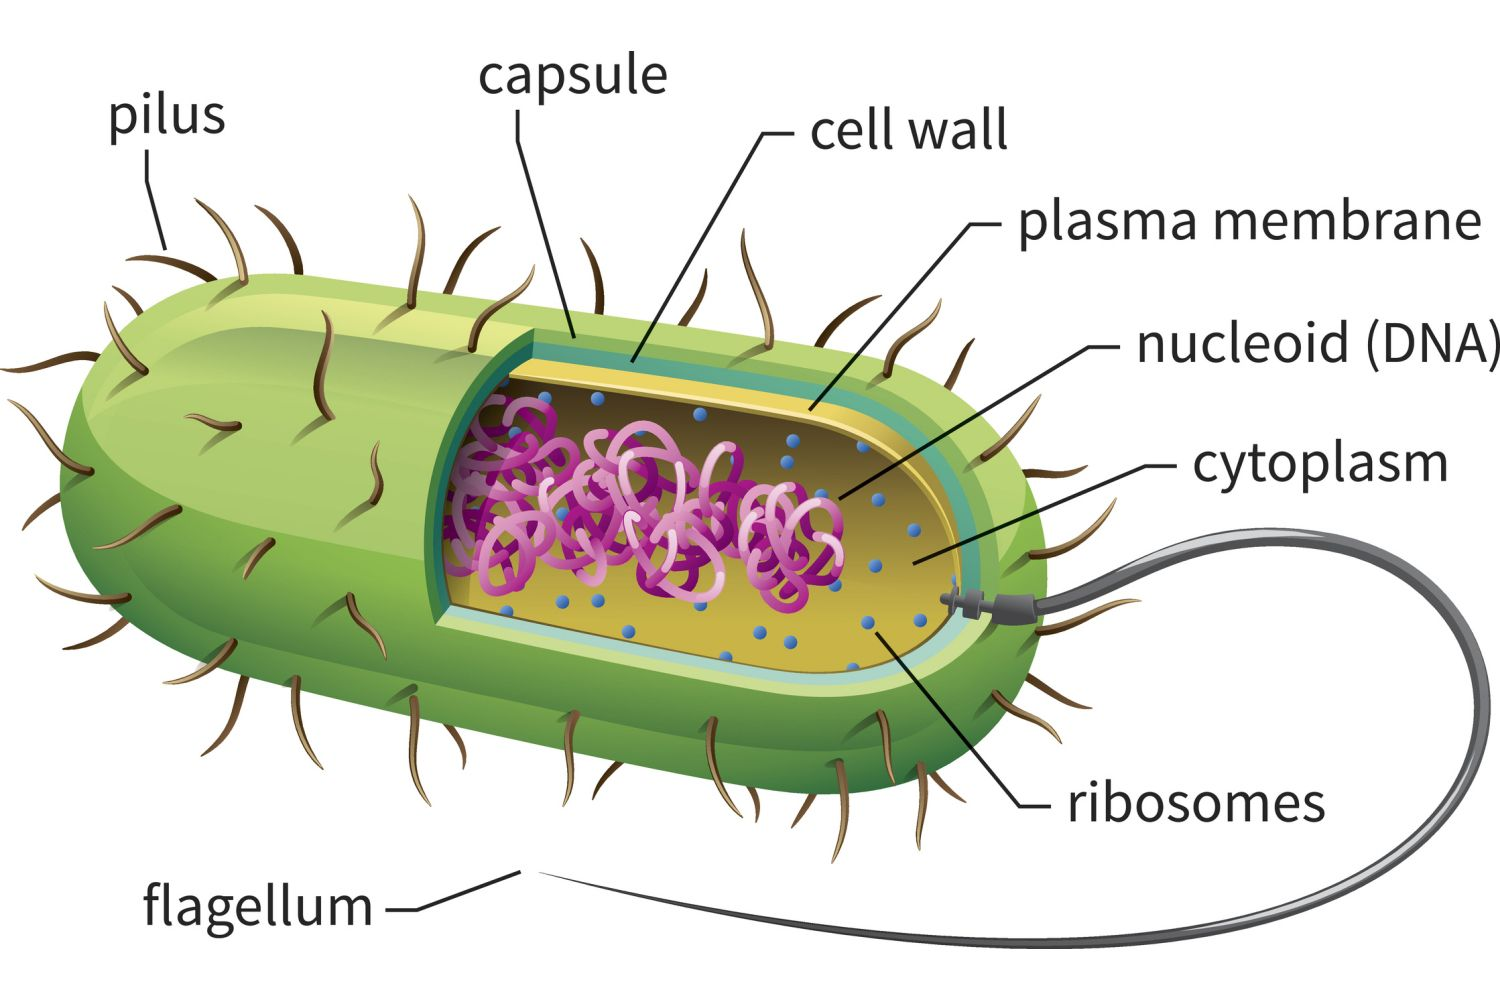
\includegraphics[width=1.0\textwidth]{figures/bacteria_cell.jpg}
			\end{center}
		\end{column}
		
		\begin{column}{0.5\textwidth}
			\begin{center}
				\textbf{Eukaryotic Cell}\\
				\vspace{0.5cm}
				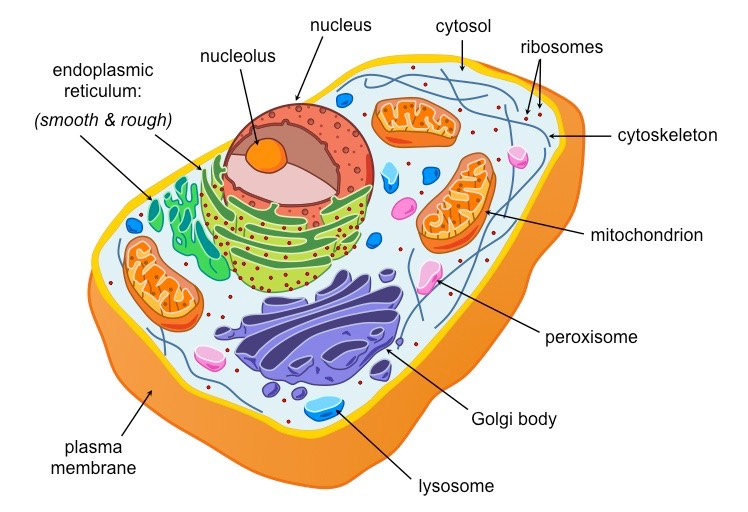
\includegraphics[width=1.0\textwidth]{figures/animal.jpg}
			\end{center}
		\end{column}
	\end{columns}
\end{frame}


%-------------------------------%
% Prokaryotes & Eukaryotes II   %
%-------------------------------%
\begin{frame}
	\begin{columns}
		\begin{column}{0.5\textwidth}
			\begin{center}
				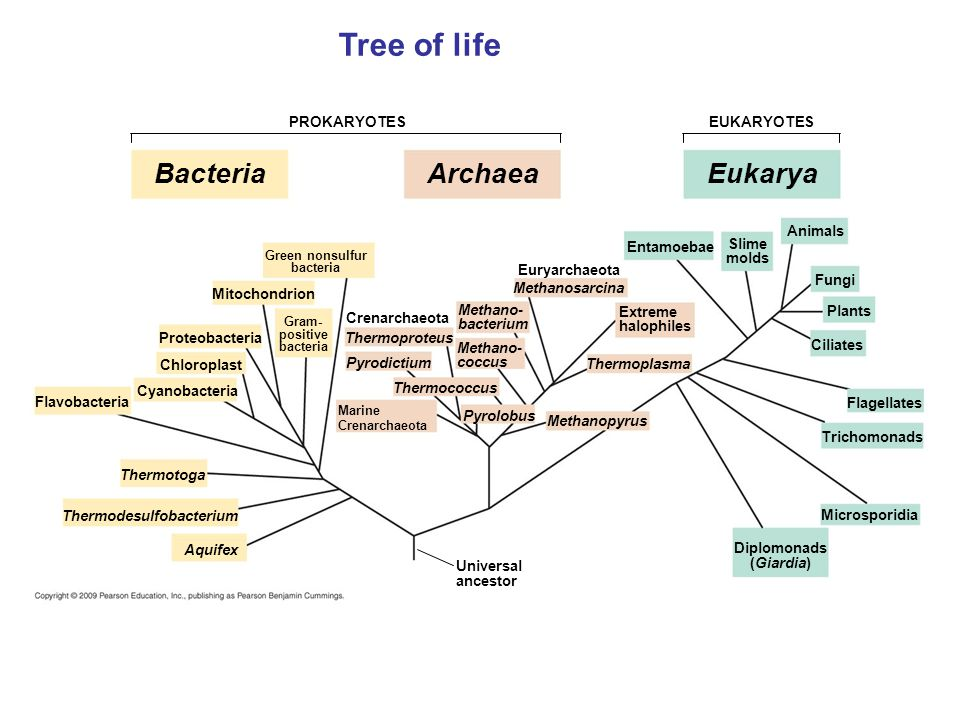
\includegraphics[width=1.0\textwidth]{figures/tree4.jpg}
			\end{center}
		\end{column}
		
		\begin{column}{0.5\textwidth}
			\begin{center}
				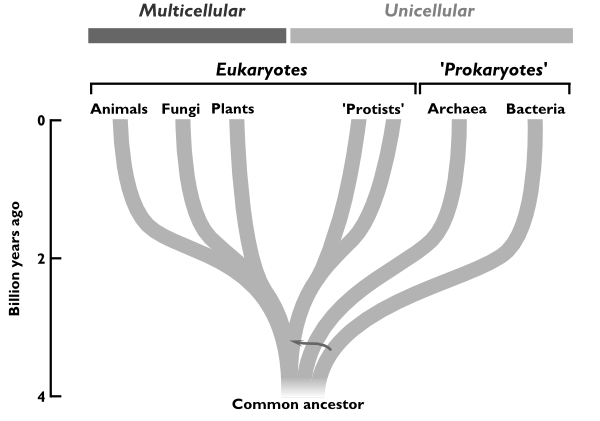
\includegraphics[width=1.0\textwidth]{figures/tree3.png}
			\end{center}
		\end{column}
	\end{columns}
\end{frame}


%-------------------------------%
% Prokaryotes & Eukaryotes III  %
%-------------------------------%
\begin{frame}[t]
\frametitle{Prokaryotes \& Eukaryotes}
\vspace{0.25cm}

	\begin{center}
		\textcolor{myblue}{How are they related?}
	\end{center}

	\vspace{0.25cm}
	
	First clue came from mitochondria:
		\medskip
		\begin{itemize}
			\item The energy producers of the cell
			\medskip
			\item About the size of a prokaryote cell
			\medskip
			\item Have their own circular DNA molecule, just like prokaryotes (that you inherit from mom)
		\end{itemize}	
	
	\begin{center}
		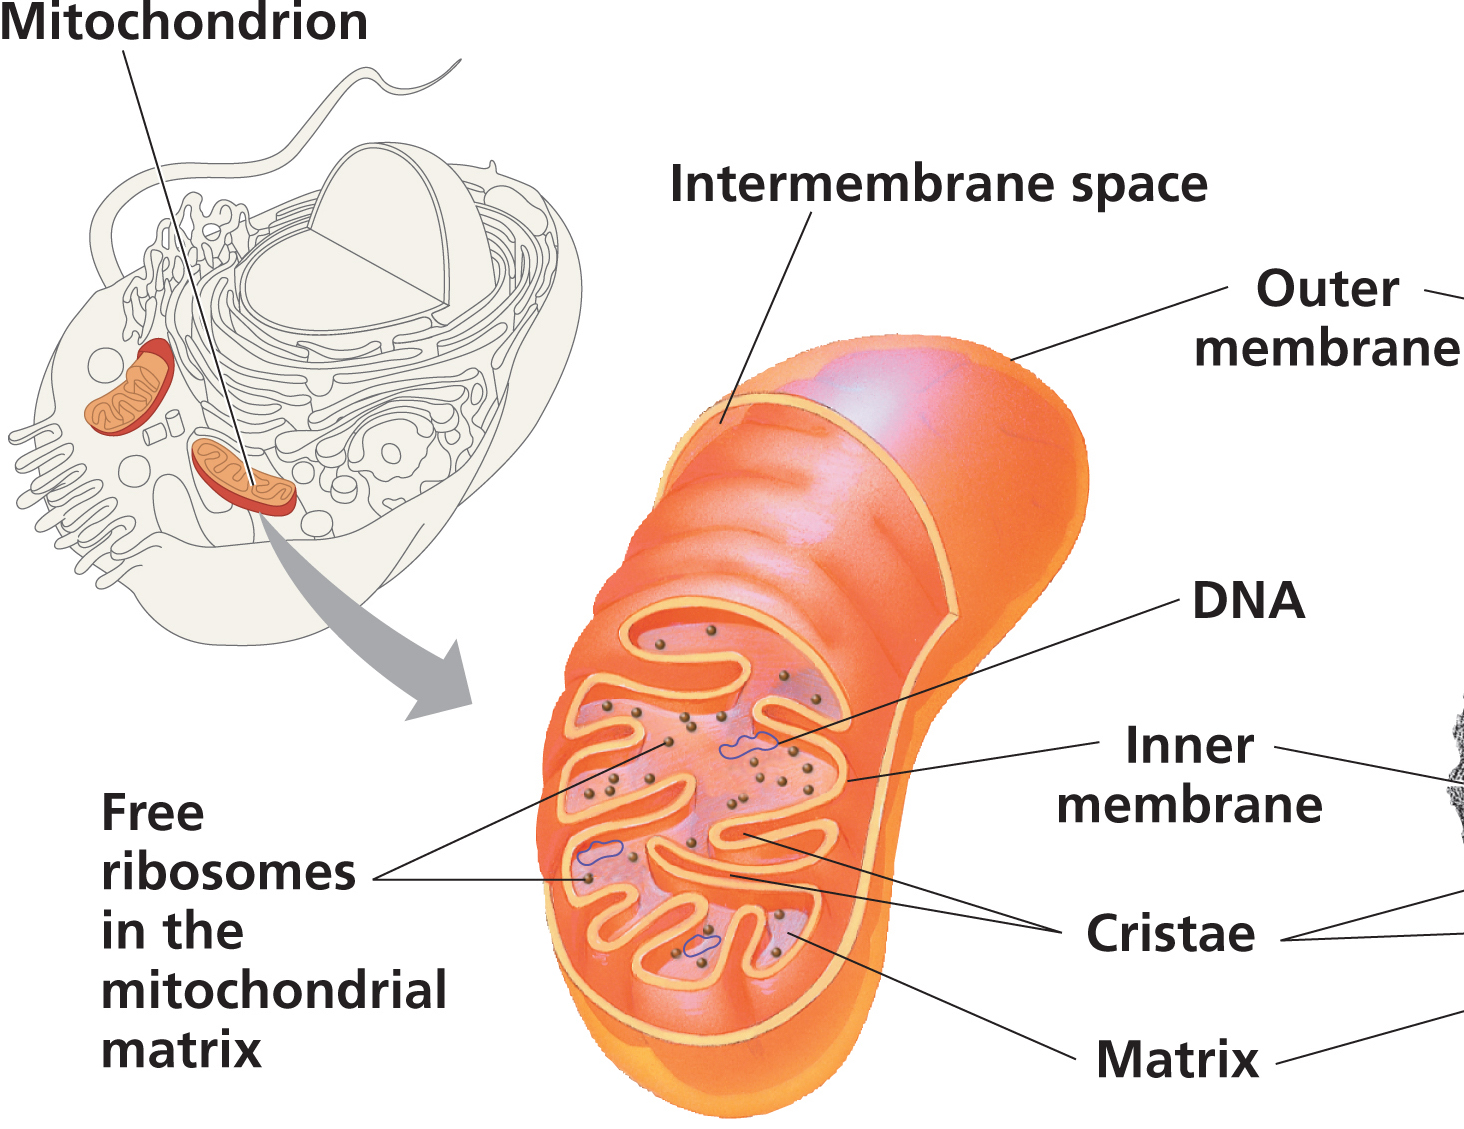
\includegraphics[width=0.4\textwidth]{figures/fg06_17a.jpg}
	\end{center}	
\end{frame}


%-------------------------------%
% Prokaryotes & Eukaryotes IV   %
%-------------------------------%
\begin{frame}[t]
\frametitle{Prokaryotes \& Eukaryotes}
\vspace{0.25cm}

	\begin{center}
		\textcolor{myblue}{How are they related?}
	\end{center}

	\vspace{0.25cm}
	
	Similar situation with chloroplasts (plants):
		\medskip
		\begin{itemize}
			\item Convert sunlight into chemical energy
			\medskip
			\item About the size of a prokaryote cell
			\medskip
			\item Have their own circular DNA molecule, just like prokaryotes (that you inherit from mom)
		\end{itemize}	
	
	\begin{center}
		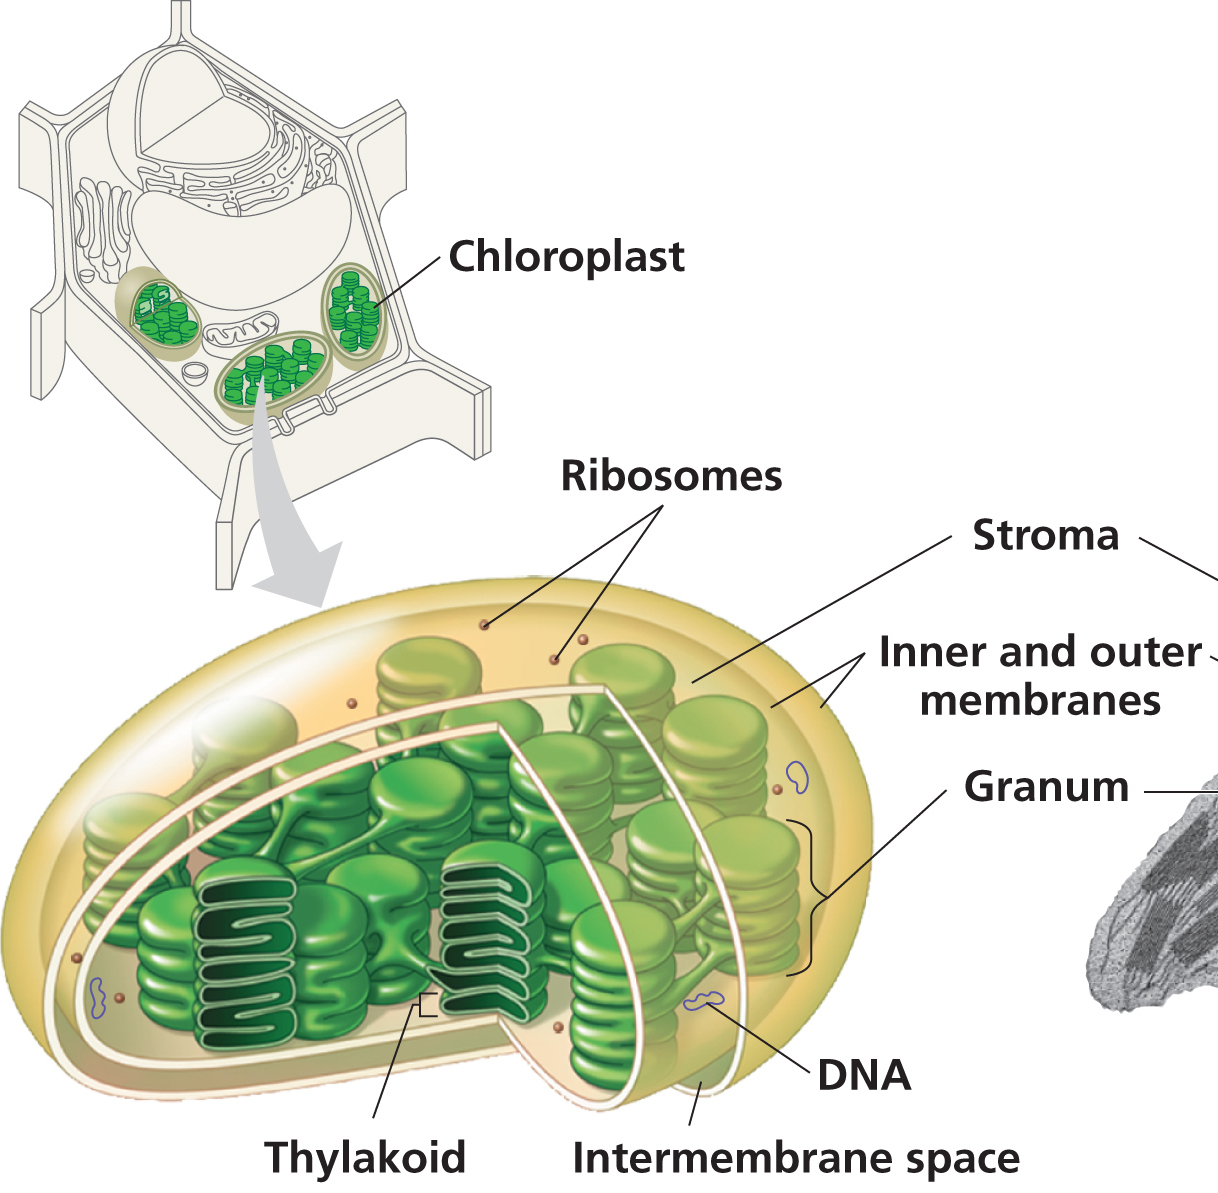
\includegraphics[width=0.4\textwidth]{figures/fg06_18.jpg}
	\end{center}	
\end{frame}


%-------------------------------%
% Prokaryotes & Eukaryotes V    %
%-------------------------------%
\begin{frame}
\frametitle{Prokaryotes \& Eukaryotes}
\framesubtitle{Endosymbiont theory}
	\begin{center}
		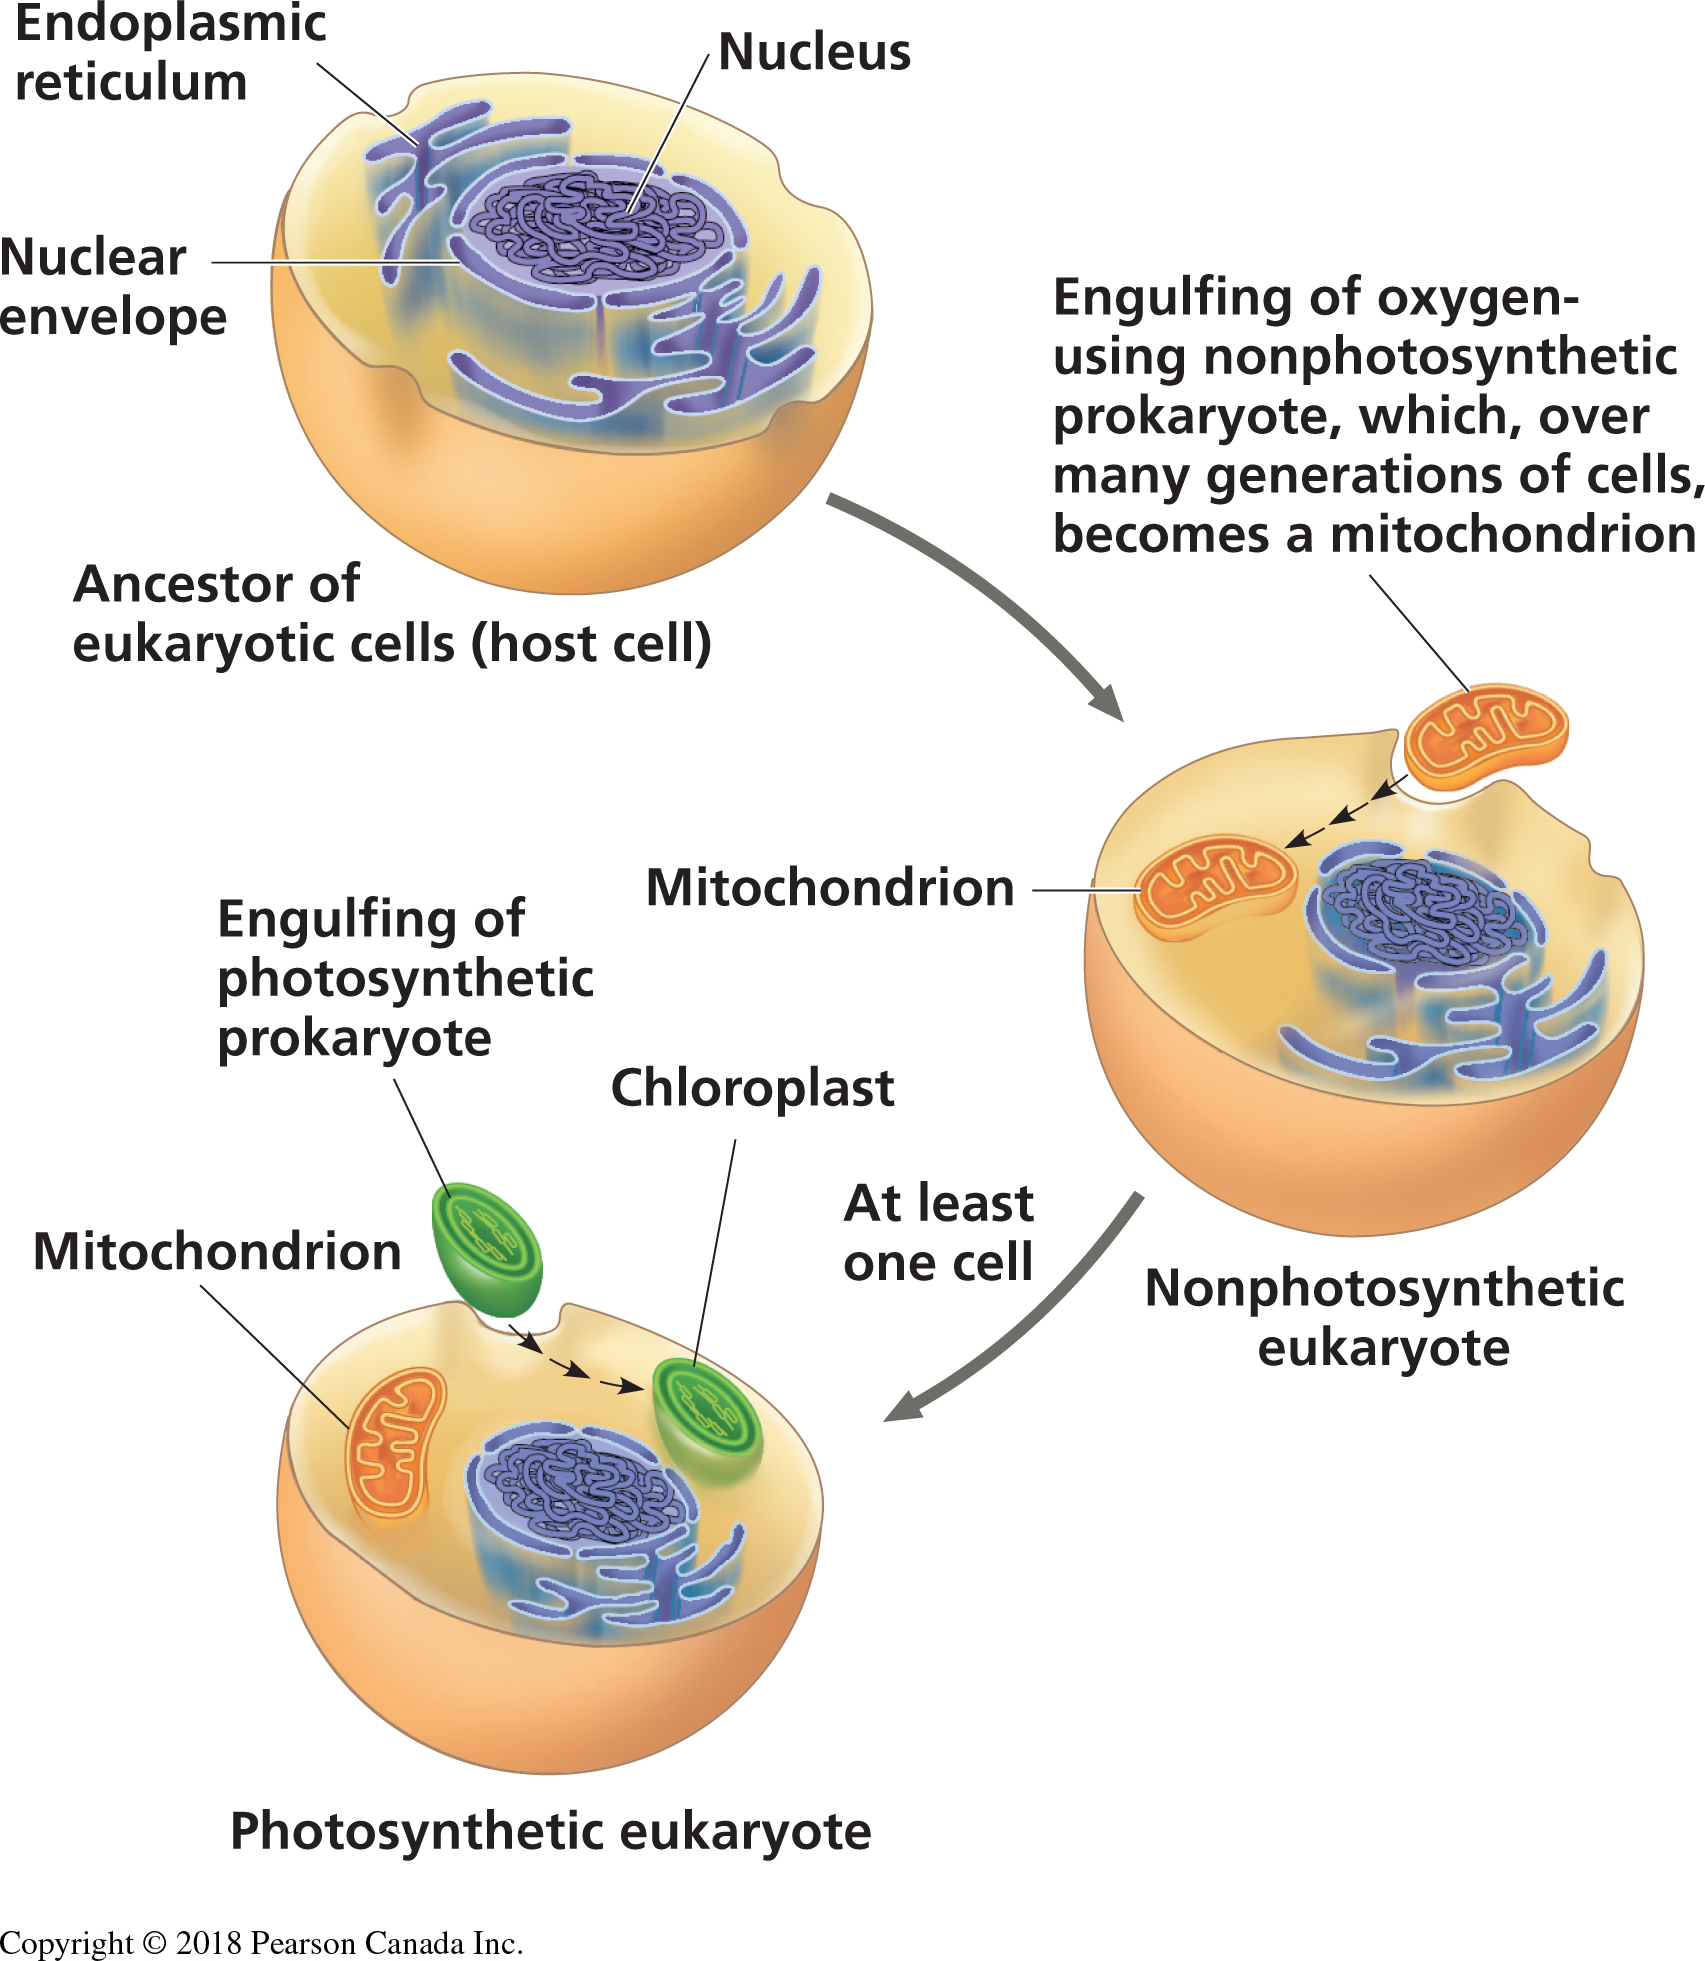
\includegraphics[width=0.55\textwidth]{figures/fg06_16.jpg}
	\end{center}	
\end{frame}


%-------------------------------%
% Prokaryotes & Eukaryotes VI   %
%-------------------------------%
\begin{frame}[t]
\frametitle{Prokaryotes \& Eukaryotes}

	\begin{reference}{4mm}{92mm}
		\rule{1.5cm}{0.25pt}\\
		From Margulis L (1970) \emph{Origin of Eukaryotic Cells}. Yale University Press.
	\end{reference}

	\begin{center}
		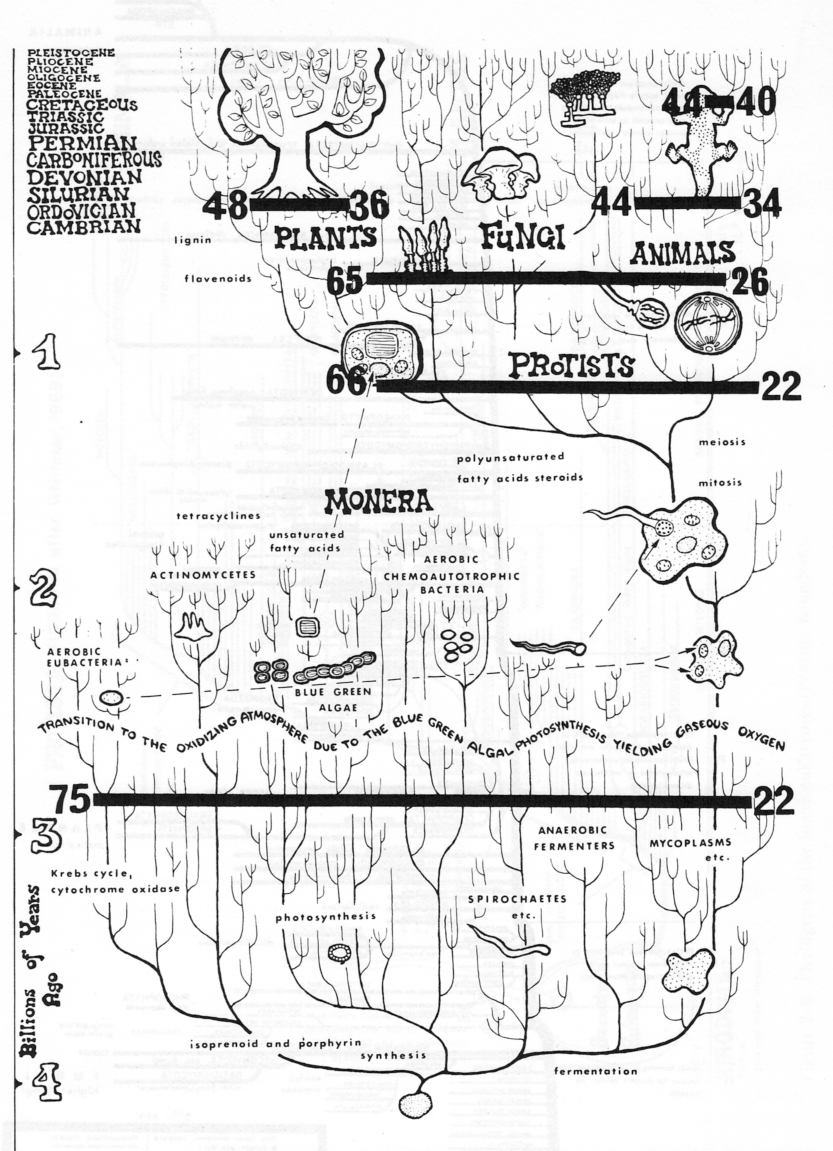
\includegraphics[width=0.5\textwidth]{figures/margulisTree.pdf}
	\end{center}
\end{frame}


%-------------------------------%
% Case Study                    %
%-------------------------------%
\begin{frame}[t]
\frametitle{Case Study}
\vspace{0.5cm}

	\begin{columns}[t]
		\begin{column}{0.5\textwidth}
			\begin{center}
				Chapter 9\\
				\vspace{0.25cm}
				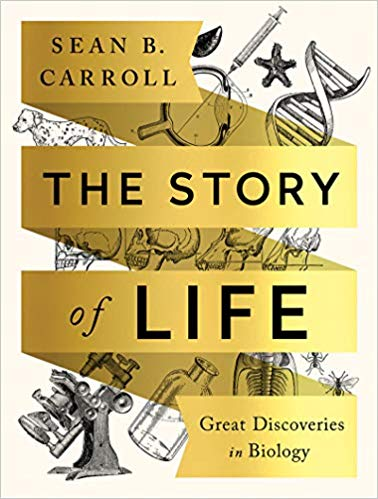
\includegraphics[width=0.6\textwidth]{../Topic1-Introduction/figures/carroll.jpg}
			\end{center}
		\end{column}
		
		\begin{column}{0.5\textwidth}
			\begin{center}
				Lynn Margulis\\
				\vspace{0.25cm}
				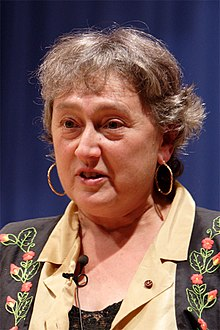
\includegraphics[width=0.6\textwidth]{figures/Margulis.jpg}
			\end{center}
		\end{column}
	\end{columns}
\end{frame}


%-------------------------------%
% Case Study II                 %
%-------------------------------%
\begin{frame}

	\begin{center}
		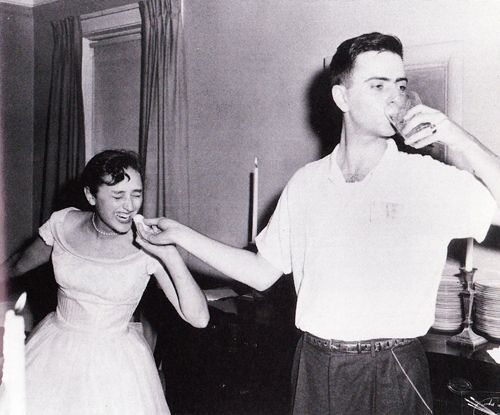
\includegraphics[width=0.8\textwidth]{figures/lynn-carl.jpg}
	\end{center}
\end{frame}


%-------------------------------%
% Case Study II                 %
%-------------------------------%
\begin{frame}

	\begin{center}
		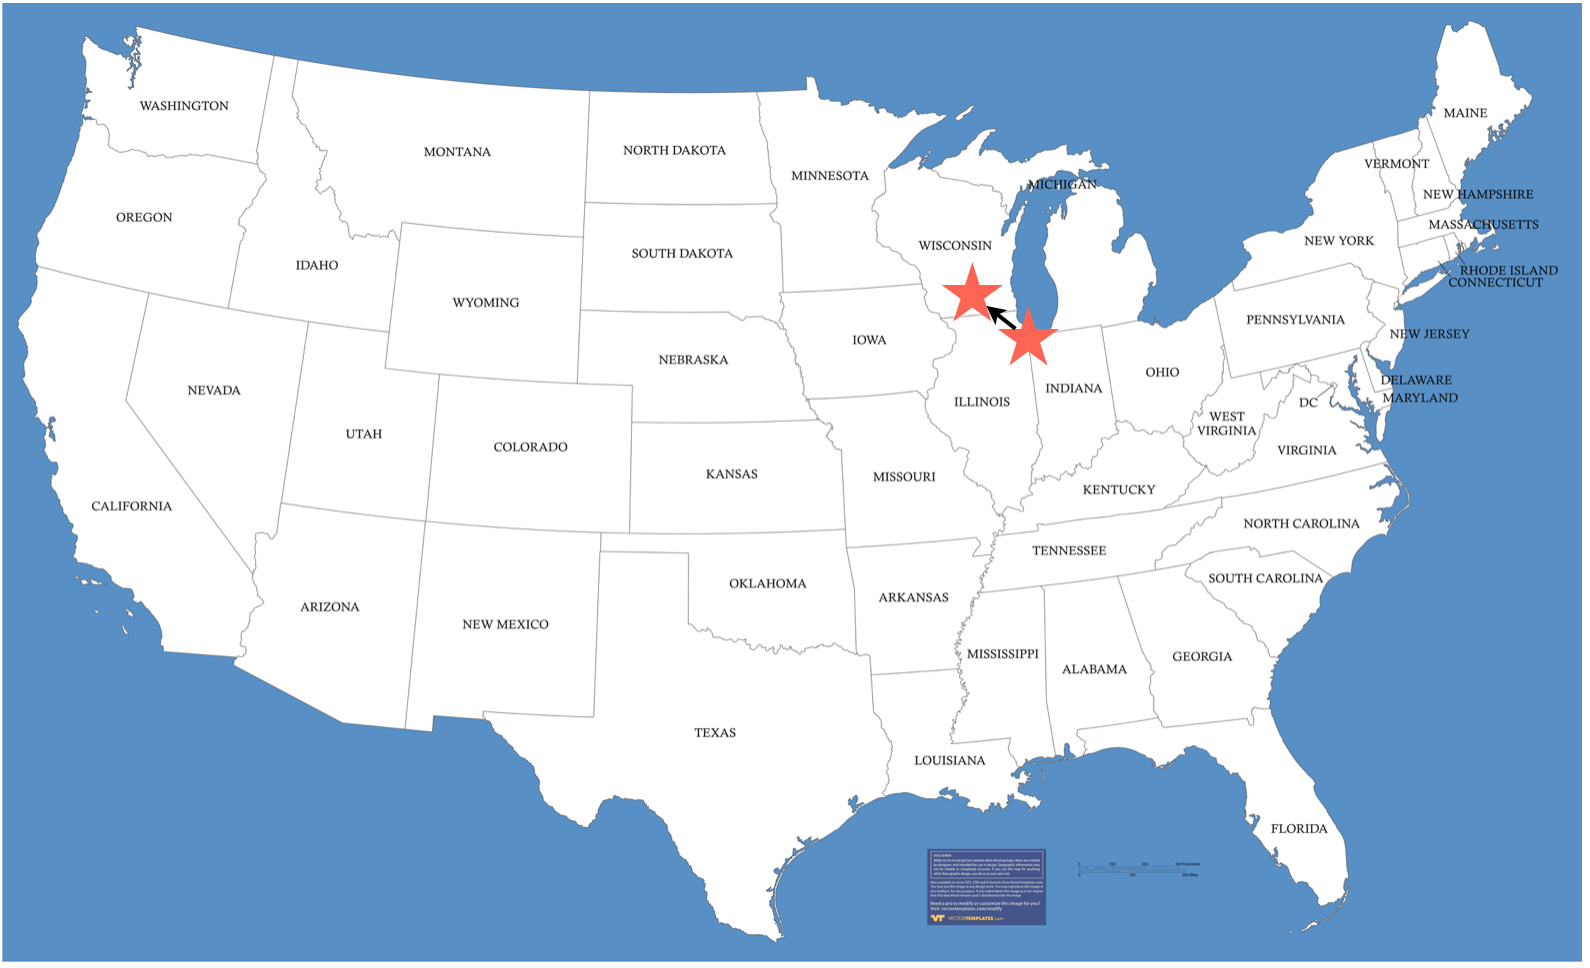
\includegraphics[width=0.8\textwidth]{figures/map1.png}
	\end{center}
\end{frame}


%-------------------------------%
% Case Study III                %
%-------------------------------%
\begin{frame}

	\begin{center}
		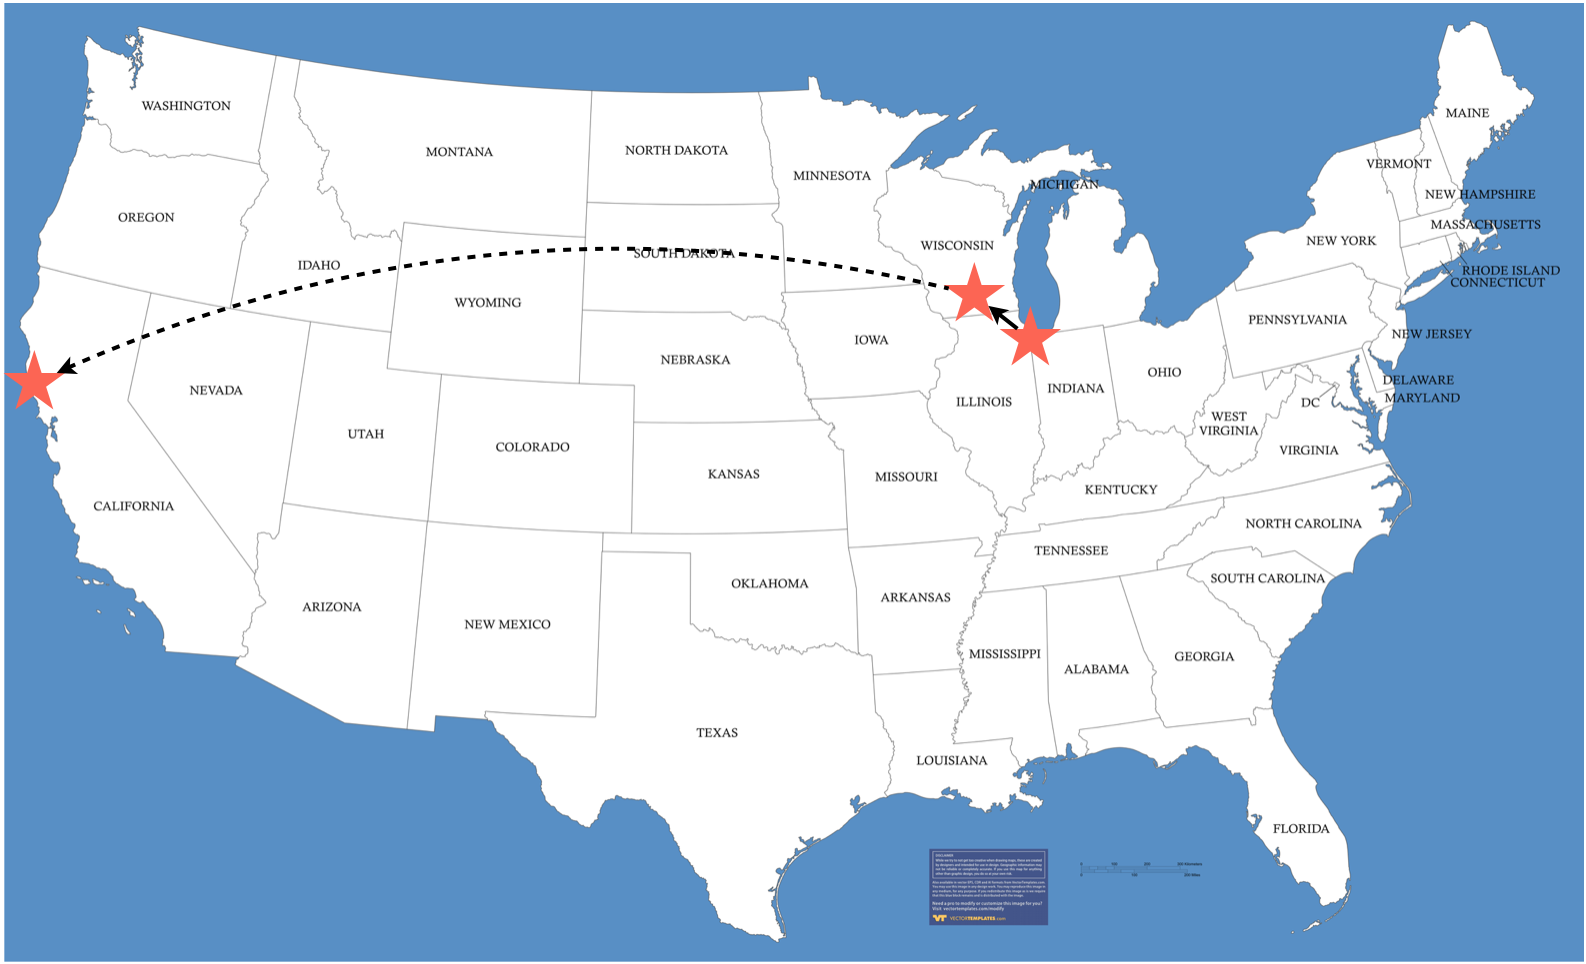
\includegraphics[width=0.8\textwidth]{figures/map2.png}
	\end{center}
\end{frame}


%-------------------------------%
% Case Study IV                 %
%-------------------------------%
\begin{frame}

	\begin{center}
		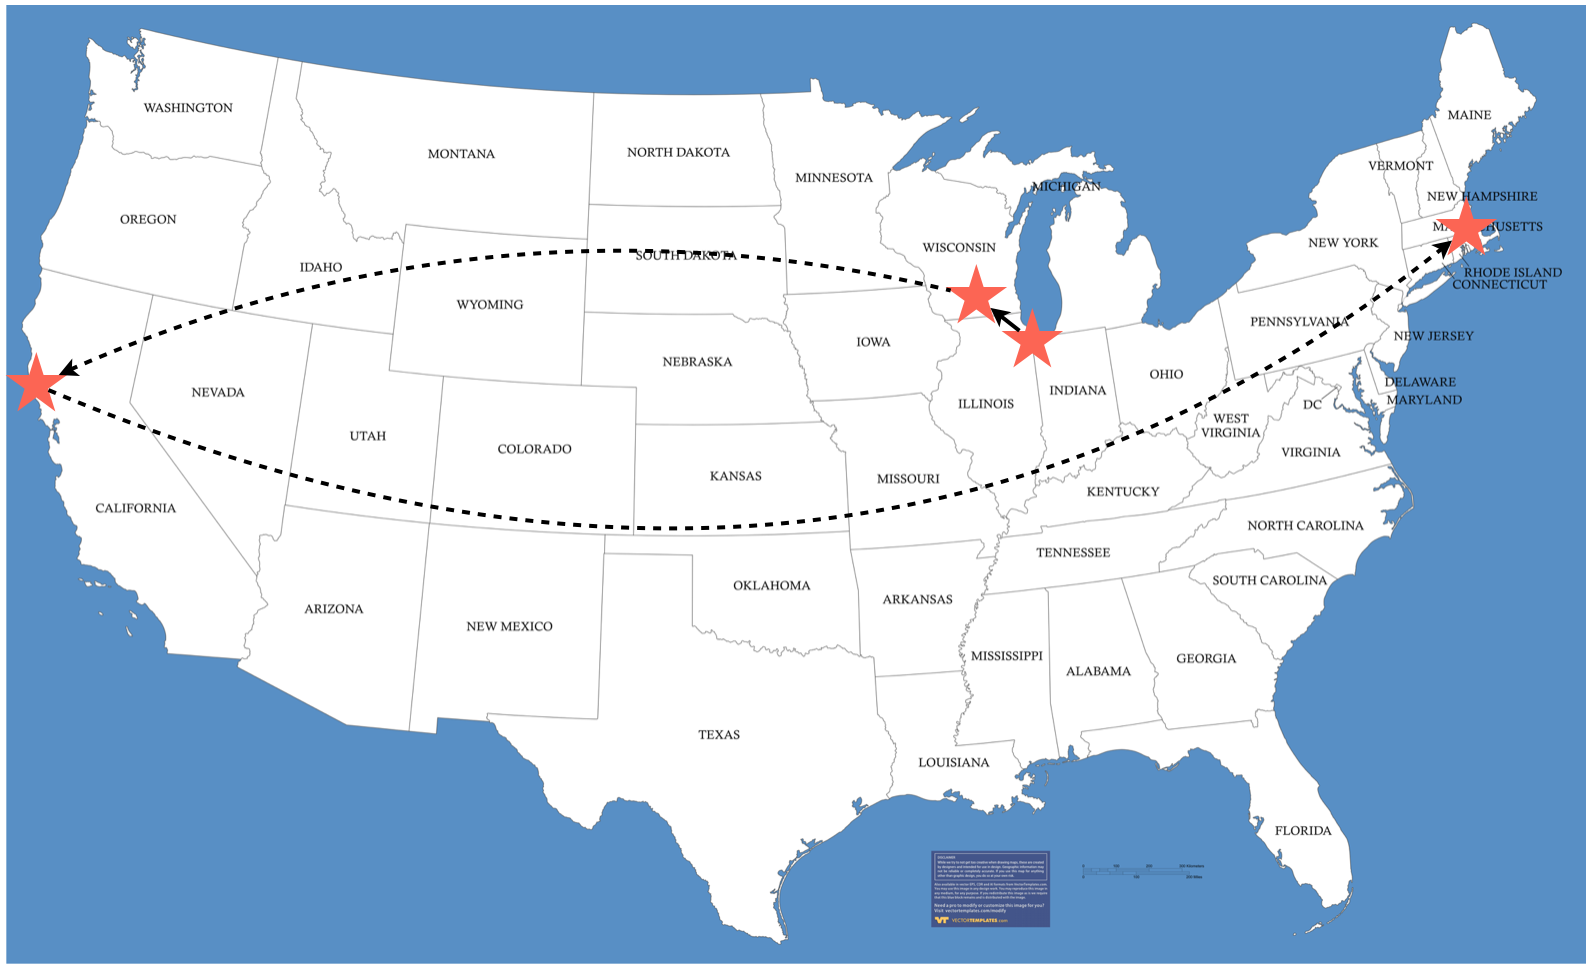
\includegraphics[width=0.8\textwidth]{figures/map3.png}
	\end{center}
\end{frame}


%-------------------------------%
% Case Study V                  %
%-------------------------------%
\begin{frame}
	\begin{center}
		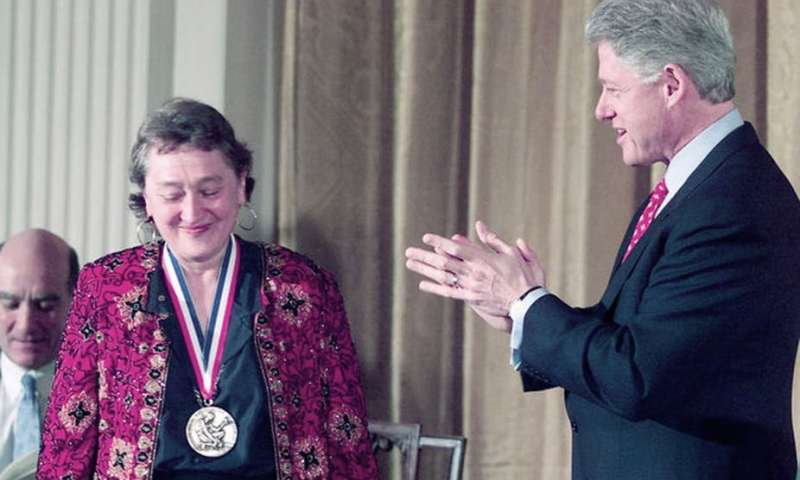
\includegraphics[width=0.8\textwidth]{figures/Margulis2.jpg}
	\end{center}
\end{frame}


%----------------------------------%
% Internal Structures: Nucleus I   %
%----------------------------------%
\begin{frame}[t]
\frametitle{Internal Structures}
\framesubtitle{1. Nucleus}
\vspace{0.25cm}

	Has 2 bilayers instead of 1
		\begin{itemize}
			\item Outer one joins ER
		\end{itemize}
	
	\vspace{0.25cm}
	
	Pores for allowing movement of molecules in and out\\
	
	\vspace{0.25cm}
	
	\textbf{Nucleolus:} Where ribosomal RNA, and ribosomes are synthesized (will come back to these later)\\
	
	\begin{columns}
		\begin{column}{0.5\textwidth}
			\textbf{Chromatin:} DNA + proteins
		\end{column}
		
		\begin{column}{0.5\textwidth}
			\begin{center}
				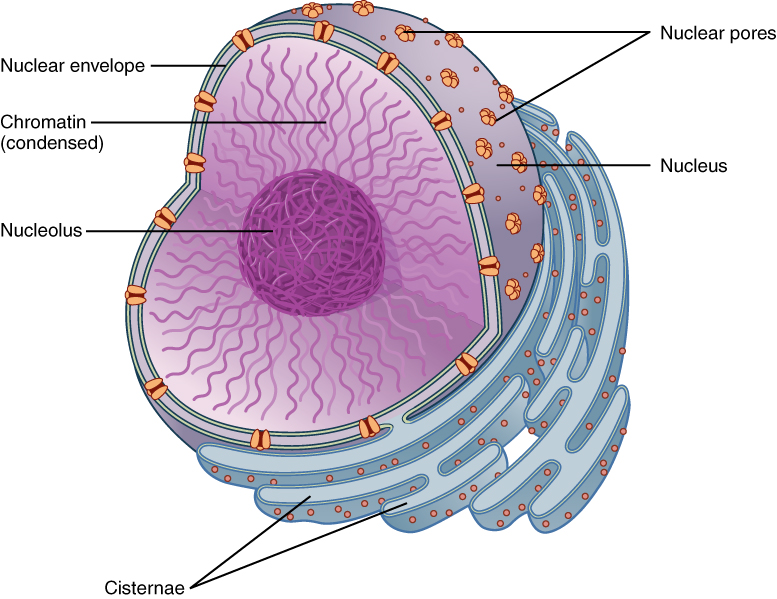
\includegraphics[width=1.0\textwidth]{figures/nucleus.jpg}
			\end{center}
		\end{column}
	\end{columns}
\end{frame}


%----------------------------------%
% Internal Structures: Rough ER    %
%----------------------------------%
\begin{frame}[t]
\frametitle{Internal Structures}
\framesubtitle{2. Rough Endoplasmic Reticulum (ER)}
\vspace{0.5cm}

	Studded with ribosomes\\
	
	\vspace{0.5cm}
	
	Where proteins are synthesized\\
	
	\vspace{0.2cm}
	
	\begin{center}
		\includegraphics[width=0.6\textwidth]{figures/roughER.jpg}
	\end{center}

\end{frame}


%----------------------------------%
% Internal Structures: Smooth ER   %
%----------------------------------%
\begin{frame}[t]
\frametitle{Internal Structures}
\framesubtitle{3. Smooth Endoplasmic Reticulum (ER)}
\vspace{0.5cm}

	Variety of functions depending on cell type, including:
		\medskip
		\begin{itemize}
			\item Synthesis of lipids
			\medskip
			\item Metabolism of carbohydrates
			\medskip
			\item Detoxification of drugs and poisons (especially in the liver)
		\end{itemize}
	
	\vspace{0.2cm}
	
	\begin{center}
		\includegraphics[width=0.6\textwidth]{figures/roughER.jpg}
	\end{center}

\end{frame}


%---------------------------------------%
% Internal Structures: Golgi Apparatus  %
%---------------------------------------%
\begin{frame}[t]
\frametitle{Internal Structures}
\framesubtitle{4. Golgi Apparatus}
\vspace{0.5cm}

	Modification and sorting of products of the ER\\
	
	\vspace{0.5cm}
	
	Each section (cisternae) a different stage of modification\\
	
	\vspace{0.2cm}
	
	\begin{center}
		\includegraphics[width=0.75\textwidth]{figures/golgi.jpg}
	\end{center}

\end{frame}


%-------------------------------------------%
% Internal Structures: Vesicles & Movement  %
%-------------------------------------------%
\begin{frame}[t]
\frametitle{Internal Structures}
\framesubtitle{5. Vesicles}
\vspace{0.5cm}

	
	\begin{center}
		\includegraphics[width=0.75\textwidth]{figures/vesicles.jpg}
	\end{center}

\end{frame}


%-------------------------------------------%
% Internal Structures: Vesicles & Movement  %
%-------------------------------------------%
\begin{frame}
\frametitle{Internal Structures}
\framesubtitle{5. Vesicles}

	
	\begin{center}
		\href{http://www.sumanasinc.com/webcontent/animations/content/vesiclebudding.html}{\LARGE{\textbf{Video}}}
	\end{center}

\end{frame}


%-------------------------------------------%
% Internal Structures: Energy               %
%-------------------------------------------%
\begin{frame}
	
	\begin{center}
		\LARGE{\textcolor{myblue}{Organelles that transform energy}}\normalsize{}\\
	\end{center}

\end{frame}


%-------------------------------------------%
% Internal Structures: Mitochondria         %
%-------------------------------------------%
\begin{frame}[t]
\frametitle{Internal Structures}
\framesubtitle{6. Mitochondria}	
\vspace{0.5cm}

		\begin{columns}
		\begin{column}{0.5\textwidth}
			Sugars and other molecules broken down into ATP\\
			\vspace{0.25cm}
			Have an inner and outer membrane\\
			\vspace{0.25cm}
			\# in cell depends on cell's function\\
			\vspace{0.25cm}
			Present in animal and plant cells\\
		\end{column}
		
		\begin{column}{0.5\textwidth}
			\centerline{\includegraphics[width=1.0\textwidth]{figures/figure_05_27_01.jpg}}
		\end{column}
	\end{columns}
\end{frame}
	
	
%-------------------------------------------%
% Internal Structures: Chloroplasts         %
%-------------------------------------------%
\begin{frame}[t]
\frametitle{Internal Structures}
\framesubtitle{7. Chloroplasts}	
\vspace{0.5cm}

		\begin{columns}
		\begin{column}{0.5\textwidth}
			Use energy from the \textcolor{orange}{sun} to synthesize simple sugars (\textbf{photosynthesis})\\
			\vspace{0.25cm}
			Like the nucleus, also have a double-membrane system\\
			\vspace{0.25cm}
			Also have an internal membrane called the \textbf{thylakoid}\\
				\begin{itemize}
					\item Contains light-collecting pigments such as \textbf{chlorophyll} - \textcolor{green}{green}
				\end{itemize}
			\vspace{0.25cm}
			Present in plants and green algae\\
		\end{column}
		
		\begin{column}{0.5\textwidth}
			\centerline{\includegraphics[width=1.0\textwidth]{figures/figure_05_28_01.jpg}}
		\end{column}
	\end{columns}
\end{frame}

\end{document}